\documentclass[12pt]{report}
\usepackage{kjfsty}

\begin{document}

\tableofcontents
\onehalfspacing

%\renewcommand{\sfdefault}{phv}
%\renewcommand{\rmdefault}{ptm}
%\renewcommand{\ttdefault}{pcr}


%\glossary{name={entry name}, description={entry description}, sort=h, format=textbf, number=section}

\glossary{name={$\hslash$}, description={Planck's constant}, sort=h}
\glossary{name={$m^*$}, description={electron effective mass, usually energy- and position-dependent \slunit{mass}}, sort=m}
\glossary{name={$z$}, description={dimension of quantum confinement}, sort=z}
\glossary{name={$V$}, description={quantum well potential, normally conduction band \slunit{volts}}, sort=v}
\glossary{name={$\EE$}, description={quantum state eigen energy}, sort=e}
\glossary{name={$\psi$}, description={one-dimensional electron wave function}, sort=2}
\glossary{name={$\rho$}, description={rho}, sort=22b}
\glossary{name={$\theta$}, description={theta}, sort=22a}
\glossary{name={$\gamma$}, description={gamma}, sort=22}
%\glossary{name={$$}, description={}, sort=}
%\glossary{name={}, description={}, sort=}


\chapter[Quantum Cascade Laser Design and Operation Theory]{Quantum Cascade Laser \\ Design and Operation Theory}
%\chaptermark{Design and Operation Theory}
%\markboth{Quantum Cascade Laser Design and Operation Theory}{Quantum Cascade Laser Design and Operation Theory}

Because of the inherent flexibility afforded by the QC concept, laser designs are highly customizable.  And to optimize a design for any particular goal or set of operating conditions, a basic understanding of the contributions of various laser parameters to performance is key.

In this chapter,  I provide the basic tools and derive the fundamental relations important to QC laser design and operation.  In sum, it is a QC laser ``toolbox'' generally applicable to most QC laser design circumstances.  Individually, the foundations for most sections of this chapter can be found in the references cited herein.  However, no single reference exists that thoroughly covers all the aspects important to QC laser design.  This chapter thus compiles knowledge garnered from a number of disparate sources.  Furthermore, where I have found no good source for elements I believe to be crucial to QC laser design, I provide a thorough, original discussion.

This theory becomes the foundation for ideas presented in later chapters, and it also provides a basis for new insights and understanding derived from the data presented in the remainder of this thesis.


%Much of the understanding herein described was gained

%Rarely does one find a thorough survey of QC laser theory collected in one place. I hope to accomplish this in this chapter.
%
%Five odd book chapters that give the equation, and discuss the result.  Which is all very useful, but they fail to justify where the dang equation comes from.  How can it be trusted?  Strive for derivations that are correct and transparent.
%
%Easy to understand equations that give intuition about the physical processes and mechanisms, for optimizing, trying new ideas, improving upon certain areas.  Also, equations that are easy to implement in a real calculation.
%
%What it is...
%A toolbox of QC design equations.
%Prepares you understand the basis/foundation/idea/premise/theory
%Compiles stuff that is in many disparate sources.
%Where there is no good source, I do it myself.
%
%What it's not...
%Doesn't rehash things that have already been done somewhere else.  Just gives main points and results.
%Isn't a cookbook for laser design.  Frankly, truly understanding QC laser design takes years of work to gain intuition under a skilled and trained mentor.  Although, erwinjr has sped up the process considerably, due to its immediate feedback.
%
%Field is dominated by experimentalists.

\section{The Schr\"{o}dinger Equation}

Fundamental to QC laser design is the ability to accurately calculate the positions of energy states in the quantum-confined dimension.  Generally, we are most interested in the conduction band wavefunctions $\psi_\tn{\tiny{C}}$.  In the elementary abstraction, we simply solve the time-independent Schr\"{o}dinger equation
\begin{equation}
\label{chpt1eqn:SEq_0}
-\frac{\hslash^2}{2m^*} \frac{\partial^2}{\partial z^2}\psi_\tn{\tiny{C}}(z) + q V_\tn{\tiny{C}}(z) \psi_\tn{\tiny{C}}(z) = \EE_q \psi_\tn{\tiny{C}}(z)
\end{equation}
where $\hslash$ is Planck's constant, $m^*$ is the conduction band effective mass, $z$ is the dimension of quantum confinement, $q V_\tn{\tiny{C}}$ is the conduction band potential energy profile, and $\EE_q$ is the eigen energy of the quantum state.
\glossary{name={$\psi_\tn{\tiny{C}}$}, description={conduction band wavefunction}, sort=123}
\glossary{name={$\hslash$}, description={Planck's constant}, sort=h}
\glossary{name={$m^*$}, description={conduction band effective mass \slunit{mass}}, sort=m}
\glossary{name={$z$}, description={dimension of quantum confinement}, sort=z}
\glossary{name={$q$}, description={fundamental charge unit}, sort=q}
\glossary{name={$V_\tn{\tiny{C}}$}, description={conduction band potential \slunit{Volts}}, sort=v}
\glossary{name={$\EE_q$}, description={eigen energy of the quantum state, usually positive if above the conduction band and negative if below}, sort=e}

Immediately, we encounter a problem.  Coupling of the conduction band energy states with the valence bands and other bands makes the solution much more complex than the simple one-band model of Eq.~\eqref{chpt1eqn:SEq_0}.  However, for our primary interest of bound conduction band solutions, these complex interactions can be reduced to an energy-dependence of the effective conduction band mass \cite{Sirtori:PRB:1994}.  Consequently, as the electron acquires more energy---\emph{i.e.} gets higher up in the band and closer to the vacuum level---the electron gets ``heavier.''  Also, our QC structure is a system of layered materials, each with a different effective mass from adjacent layers.  So, the effective mass is both energy- and position-dependent: $m^*(z,\EE)$.  This results in a small change to the simple Schr\"{o}dinger equation.  When solving the Schr\"{o}dinger equation, we are taught to match $\psi_\tn{\tiny{C}}(z)$ and $\frac{\partial}{\partial_z} \psi_\tn{\tiny{C}}(z)$ at the boundaries.  Now, with variable effective masses, the solutions of envelope functions \cite{Harrison} are continuous across material interfaces in both $\psi_\tn{\tiny{C}}(z)$ and $\frac{1}{m^*} \frac{\partial}{\partial z} \psi_\tn{\tiny{C}}(z)$.
\glossary{name={$m^*(z,\EE)$}, description={energy- and position-dependent effective mass}, sort=m}

Because of variable effective mass, the classical portrayal of the Schrodinger equation is somewhat different.  Given the momentum operator $\mathcal{P}_z = -\rm{i} \hslash \partial_z$, the kinetic energy operator $\mathcal{T}$ becomes \cite{Sirtori:PRB:1994}
\begin{equation}
\mathcal{T} = \mathcal{P}_z \frac{1}{2 m^*(z,\EE)} \mathcal{P}_z =
-\frac{\hslash^2}{2} \frac{\partial}{\partial z} \frac{1}{m^*(z,\EE)} \frac{\partial}{\partial z}
\end{equation}
\glossary{name={$\mathcal{P}_z$}, description={momentum operator}, sort=p}
\glossary{name={$\mathcal{T}$}, description={kinetic energy operator}, sort=k}
and the Schr\"{o}dinger equation now becomes
\begin{equation}
\label{chpt1eqn:SEq_1}
-\frac{\hslash^2}{2} \frac{\partial}{\partial z} \frac{1}{m^*(z,\EE)} \frac{\partial}{\partial z} \psi_\tn{\tiny{C}}(z) + V_\tn{\tiny{C}}(z) \psi_\tn{\tiny{C}}(z) = \EE_q(z) \psi_\tn{\tiny{C}}(z)
\end{equation}
where $\EE_q(z)$ acquires a position-dependence when defined as the energy relative to the conduction band edge and in the presence of an applied electric field $E_\textit{field}$.  Now, to make Eq.~\eqref{chpt1eqn:SEq_1} discrete, we approximate the derivative as
\begin{equation}
\label{chpt1eqn:discrete_derivative}
\frac{d \tn{f}}{dz} \approx \frac{\Delta \tn{f}}{\Delta z} = \frac{\tn{f}(z+\delta z) -\tn{f}(z-\delta z)}{2 \delta z} \text{~.}
\end{equation}
\glossary{name={$E_\tn{\textit{field}}$}, description={applied electric field}, sort=e}
%and
%\begin{equation}
%\begin{split}
%\frac{\textrm{d}^2 f}{\textrm{d} z^2} \approz \frac{\frac{\textrm{d} f}{\textrm{d} z}\right \big |_{z+\delta z} - \frac{\textrm{d} f}{\textrm{d} z}\right \big |_{z-\delta z}}{2 \delta z} &= \frac{f(z+2 \delta z) -2 f(z) + f(z-2 \delta z)}{(2 \delta z)^2}\\
%&\Rightarrow \frac{f(z+\delta z) -2 f(z) + f(z-\delta z)}{(\delta z)^2}
%\end{split}
%\end{equation}
The Schr\"{o}dinger equation above can be discretized by expanding $\mathcal{T} \psi_\tn{\tiny{C}}(z)$.
\begin{equation}
\frac{\frac{1}{m^{*}(z+\delta z,\EE)} \frac{\partial \psi(z)}{\partial z} \big |_{z+\delta z} - \frac{1}{m^{*}(z-\delta z,\EE)} \frac{\partial \psi(z)}{\partial z} \big |_{z-\delta z}}{2 \delta z} = \frac{2}{\hslash^2}[q V_\tn{\tiny{C}}(z)-\EE]\psi_\tn{\tiny{C}}(z)
\end{equation}
Applying Eq.~\eqref{chpt1eqn:discrete_derivative} to the above equation, gathering terms in $\psi(z)$, and making the transformation $2 \delta z \rightarrow \delta z$ gives
\begin{equation}
\label{chpt1eqn:numerical_S_eq}
\begin{split}
\psi_\tn{\tiny{C}}(z+\delta z) &= \Biggl\{ \left[ \frac{2(\delta z)^2}{\hslash^2} [q V(z)_\tn{\tiny{C}}-\EE]+\frac{1}{m^{*}(z+\delta z/2,\EE)}+\frac{1}{m^{*}(z-\delta z/2,\EE)} \right] \psi(z) \qquad \qquad\\
& \qquad \qquad \qquad \qquad  - \frac{1}{m^{*}(z-\delta z/2,\EE)} \psi(z-\delta z) \Biggr\} m^{*}(z+\delta z/2,\EE)
\end{split}
\end{equation}
The effective mass at the intermediate points $z\pm \delta z/2$ is found by taking the average of the effective mass for the two adjacent points $z$ and $z+\delta z$.  By virtue of having coupled quantum well structures with abrupt material interfaces and the presence of varying electric fields, all parameters related to wavefunctions, energies, effective masses, etc.\ will be implicitly assumed to have position-dependence $z$, and these references will be hereafter dropped when not explicitly needed.
\glossary{name={$\delta z$}, description={discrete step size in $z$}, sort=104}

The shooting method is used to solve for the eigen energies of our system through the application of Eq.~\eqref{chpt1eqn:numerical_S_eq}.  Specifically, we look for bound solutions of the system confined by the dimensions $z=0$ and $z=z_{end}$.  That is, any energy $\EE$ where $\psi(0)=0$ and $\psi(z_{end})=0$.  In an elementary implementation of the shooting method, the energy space covered by our potential $V_\tn{\tiny{C}}(z)$ is initially divided into many discrete steps.  Then, Eq.~\eqref{chpt1eqn:numerical_S_eq} is used to propagate through discrete steps in $z$ to find $\psi(z_{end})$ for each initial energy value, where the initial conditions $\psi(0)=0$ and $\psi(z_\textit{second})=1$  are used ($z_\textit{second}$ being the second discrete solve point after $z=0$).  To find the exact energy value of a bound solution, we take advantage of the fact that $\psi(z_{end})$ switches signs at a bound solution.  Therefore, when $\psi(z_{end})$ is plotted for all energies over our energy space, noting the location in energy of a sign flip of $\psi(z_{end})$, allows us to iterate in energy around this point to find the exact value of the bound solution.  Figure~\ref{chpt1:shooting_example} provides an example; here, our potential $V_\tn{\tiny{C}}(z)$ is for a single quantum well in the \InGaAs / \AlInAs system, with conduction band offset of 520~meV, and an applied electric field $E_\textit{field}=25$~kV/cm.  Four bound solutions are found, and $\psi_tn{\tiny{C}}(z)$ is plotted for each solution, using the eigen energy as the baseline of the wavefunction.
\glossary{name={$z_\tnit{second}$}, description={second discrete solve point after $z=0$}, sort=z}
\glossary{name={$z_{end}$}, description={final discrete point in a confined system}, sort=z}

\begin{figure}[tp]
\centering
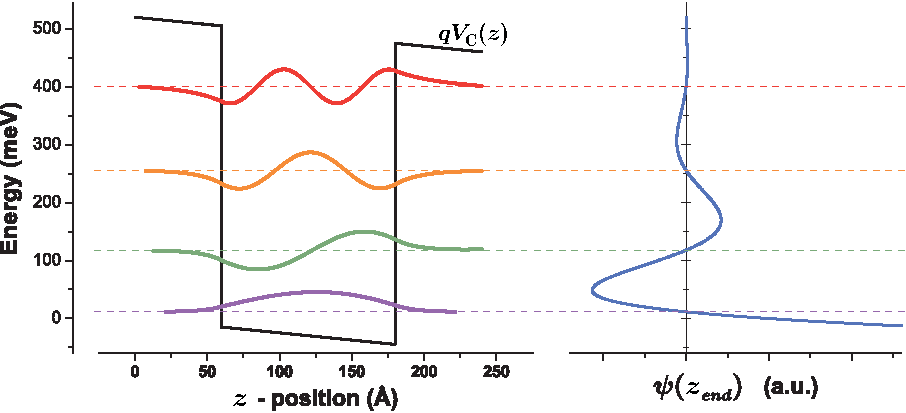
\includegraphics[width=5.5in]{shooting_ex}
\caption[Example use of the shooting method]{\tn{\textbf{Example use of the shooting method.}}  The left panel shows a potential $V(z)$ for an \InGaAs / \AlInAs quantum well with $E_\tn{\textit{field}}=25~\tn{kV/cm}$.  Four bound solutions are found by finding the roots of $\psi(z_{end})$, as shown in the right panel. The wavefunction $\psi(z)$ is plotted for the four bound solutions.}
\label{chpt1:shooting_example}
\end{figure}


\section{Interface Energy Offsets and Bandgaps}

To properly use Eq.~\eqref{chpt1eqn:numerical_S_eq} solving the time-independent Schr\"{o}dinger equation, we need accurate knowledge of two key parameters: $V_\tn{\tiny{C}}(z)$ and $m^*(z,\EE)$.  This section is devoted to attaining the band offset values that are so important to coupled quantum well systems such as QC lasers.  In the following section, we discuss effective mass in semiconductor systems.  This section and the remaining sections in this chapter make heavy use of semiconductor materials parameters; a superb review of important III--V material parameters was published by Vurgaftman \emph{et al.} in 2001 \cite{Vurgaftman}.

All QC laser implementations to date have used intersubband transitions in the conduction band.  While QC electroluminescence has been shown from valence intersubband transitions \cite{Dehlinger:Science:2000:Sige} \cite{Malis:APL:2006}, we are more keenly interested in the conduction band edge offsets of materials.  As it turns out, the valence band offsets have been much more extensively studied \cite{Vurgaftman}, owing to the experimental difficulty of measuring conduction band offsets.  When considering a valence band offset, the convention is to report the parameter $VBO$, which is the valence band offset relative to a predetermined a reference material where $VBO$ is specified as 0 (\emph{i.e.} $VBO=0$); Vurgaftman \emph{et al.}, for example, define $VBO(\tn{InSb})=0$.  In this way, the valence band offset for any arbitrary two materials is easily found as the difference in $VBO$ for the two materials of the set.  By adding the bandgap of each material to its respective $VBO$, the conduction band offset for a two material system can likewise be calculated.  More concretely, the conduction band edge (at the $\Gamma$ point) $\EE_c^\Gamma$ can be defined as
\begin{equation}
\EE_c^\Gamma = VBO + \EE_g^\Gamma + \delta\!\EE_\textit{Varsh} + \delta\!\EE_{\varepsilon c} + \delta\!\EE_{\varepsilon v}
\end{equation}
where $\EE_g^\Gamma$ is the energy gap at the $\Gamma$ point at $T=0$~K without strain, $\delta\!\EE_\textit{Varsh}$ is the Varshney correction to the bandgap energy for $T\neq0$~K, and $\delta\!\EE_{\varepsilon c}$ and $\delta\!\EE_{\varepsilon v}$ are corrections to the conduction and valence band edges due to hydrostatic deformation (\emph{i.e.} strain).  Each of these terms is treated in the following sections.  With this definition of $\EE_c^\Gamma$, the conduction band offset at the interface between two materials $A$ and $B$ is $\Delta\!\EE_c^\Gamma=\EE_c^\Gamma(A)-\EE_c^\Gamma(B)$.

\glossary{name={$VBO$}, description={valence band offset}, sort=v}
\glossary{name={$\EE_c^\Gamma$}, description={the conduction band edge at the $\Gamma$ point}, sort=e}
\glossary{name={$\EE_g^\Gamma$}, description={energy gap at the $\Gamma$ point at $T=0$~K without strain}, sort=e}
\glossary{name={$\delta\EE_\tn{\textit{Varsh}}$}, description={Varshney correction to the bandgap energy for $T\neq0$~K}, sort=104}
%\glossary{name={$\delta\!\EE_{\varepsilon v}$}, description={correction to the valence band edge due to hydrostatic deformation}, sort=104}
%\glossary{name={\delta\!\EE_{\varepsilon c}$}, description={correction to the conduction band edge due to hydrostatic deformation}, sort=104}
\glossary{name={$\Delta\EE_c^\Gamma$}, description={conduction band offset at the $\Gamma$ point}, sort=104}



\subsection{Materials parameters for ternary alloys}

Fundamental materials parameters, $VBO$ and $\EE_g^\Gamma$ for example, can be conveniently reported in tabular form for binary semiconductors, as in the review by Vurgaftman \emph{et al.} \cite{Vurgaftman}.  Ternary alloys, however, have a degree of freedom in material composition, making tabular recording prohibitive.  For any ternary material $A_x B_{1-x} C$, composed proportionally of the two constituent binaries $(AC)_x$ and $(BC)_{1-x}$, a range of values exists over the mole fraction $x$ for any generic material parameter $P$.  Conveniently, we can make use of the composition endpoints $x=0$ and $x=1$ to bound the possible values of $P$.  Then, $P$ can thus be defined as
\begin{equation}
P(A_x B_{1-x} C) = x P(AC) + (1-x) P(BC) + x(1-x) C_B
\end{equation}
where $C_B$ is the ``bowing parameter'' specific to material $ABC$.  Commonly, the bowing parameter is either not well known, or no bowing parameter exists.  In the case of $C_B=0$, the material parameter is just a linear interpolation between the value of the parameter for the two component binaries weighted by $x$.

\glossary{name={$P$}, description={generic material parameter}, sort=p}
\glossary{name={$C_B$}, description={bowing parameter}, sort=c}
\glossary{name={$x$}, description={mole fraction}, sort=x}

%kale

\begin{table}[tp]
\centering
\begin{minipage}[c]{4in}
\captionsetup{width=4in}
\centering
\setstretch{1.2}
\caption[Material parameters: InAs, GaAs, and AlAs]{Material parameters for the binary alloys InAs, GaAs, and AlAs. Source is \cite{Vurgaftman}, unless otherwise indicated.  Lattice constants are given for $300~\tn{K}$.  The effective mass is given for the bulk band edge, with $m_0$ the free electron mass.}
\vspace{-0.1in}
\begin{tabular*}{4in}{@{\extracolsep{\fill}} c c c c }%{@{\extracolsep{\fill}} c c p{0.5in} c c }
\toprule
  & InAs & GaAs & AlAs\\
\hline
$a_{\ell c}$ (\AA)  & 6.0583 & 5.6533 &  5.6611\\
$c_{11}$ (GPa)  & 832.9 & 1221 & 1250\\
$c_{12}$ (GPa)  & 452.6 & 566 & 534\\
$\EE_{G}^\Gamma$ (eV)  & 0.417 & 1.519 & 3.099\\
$\Delta_{SO}$ (eV)  & 0.39  & 0.341  & 0.28\\
$VBO$ (eV)& -0.59 & -0.80 & -1.33\\ %  \citesec{Wei:APL:1998}
$a_c^\Gamma$ (eV)  & -5.08 & -7.17 &  -5.64\\
$a_v$ (eV) &  -1.00 & -1.16 & -2.47\\
$b$ (eV)    &  -1.8 & -2.0 & -2.3\\
$\EE_P$ (eV)    &  21.5 & 28.8 & 21.1\\
$F$    &  -2.90 & -1.94 & -0.48\\
$m_e^\Gamma/m_0$  & 0.026 & 0.067 & 0.15\\
$\alpha^\Gamma$ (meV/K)  & 0.276 & 0.5405 & 0.885\\
$\beta^\Gamma$ (K)  & 93 & 204 & 530\\
$\epsilon_{s}$ & 14.3\sup{(1)} & 12.90\sup{(1)} & 10.06\sup{(1)}\\
$\epsilon_\infty$ & 11.6\sup{(1)} & 10.86\sup{(1)}  & 8.16\sup{(1)}\\
$\hslash \omega_{LO}$ & 29.93\sup{(1)} & 35.3\sup{(1)} & 49.8\sup{(1)}\\% \citesec{iivi:11}
\hline
\end{tabular*}
\singlespacing
\raggedright
\vspace*{-0.18in}
\footnotesize{(1) Ref. \cite{Adachi:book:2005}}
\label{chpt1:binary_table}
%\bibliographystylesec{kale1}
%\bibliographysec{biblio_iivi}
\end{minipage}
\end{table}

\begin{table}[tp]
\centering
\begin{minipage}[c]{2.8in}
\captionsetup{width=2.8in}
\centering
\setstretch{1.2}
\caption[Material bowing parameters: InGaAs and AlInAs]{Non-zero bowing parameters $C_B$ for the ternary alloys InGaAs and AlInAs. Source is \cite{Vurgaftman}.}
\vspace{-0.1in}
\begin{tabular*}{2.8in}{@{\extracolsep{\fill}} c c c c }%{@{\extracolsep{\fill}} c c p{0.5in} c c }
\toprule
  & InGaAs & AlInAs\\
\hline
$\EE_{G}^\Gamma$ (eV)  & 0.477 & 0.70 \\
$\Delta_{SO}$ (eV)  & 0.15 & 0.15  \\
$VBO$ (eV)& -0.38 & -0.64 \\ %
$\EE_P$ (eV)   &  -1.48 & -4.81 \\
$F$    &  1.77 & -4.44 \\
$m_e^\Gamma/m_0$  & 0.0091 & 0.049 \\
$a_c^\Gamma$ (eV)  & 2.61 & -1.4 \\
\hline
\end{tabular*}
\singlespacing
\raggedright
\vspace*{-0.18in}
%\footnotesize{(1) Ref. \cite{Adachi:book:2005}}
\label{chpt1:ternary_table}
%\bibliographystylesec{kale1}
%\bibliographysec{biblio_iivi}
\end{minipage}
\end{table}

\subsection{Temperature effects on bandgap}

The temperature dependence of semiconductor bandgaps is commonly described with the Varshni formula.  This is an empirical formula that fits two Varshni parameters---$\alpha$ [$\frac{\tn{energy}}{\tn{temperature}}$] and $\beta$ [$\tn{\footnotesize{temperature}}$]---to experimentally obtained values of bandgap with temperature.  The Varshni formula gives the temperature $T$ dependence of the bandgap as \cite{Varshni:Physica:1967}
\begin{equation}
\EE_g(T) = \EE_g(T=0)-\frac{\alpha T^2}{T+\beta}
\end{equation}
so that the temperature correction to the conduction band edge is
\begin{equation}
\delta\!\EE_\textit{Varsh}= -\frac{\alpha T^2}{T+\beta} \text{~.}
\end{equation}
The Varshney corrections for the common QC materials \InGaAs and \AlInAs are plotted in Fig.~\ref{chpt1:varsh_correc}.

\begin{figure}[tp]
\centering
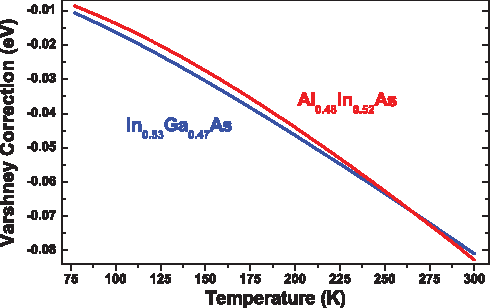
\includegraphics[width=4.5in]{chpt1_varshcorrec}
\caption[Bandgap temperature dependence]{\tn{\textbf{Bandgap temperature dependence.}}  The Varshney correction $\delta\!\EE_\tn{\textit{Varsh}}$ is plotted for the InP-lattice-matched compositions \InGaAs and \AlInAs.  The effect of increasing temperature is the lowering of the material bandgap.}
\label{chpt1:varsh_correc}
\end{figure}

\subsection{Strain effects on bandgap and band offset}

Strain in epitaxially-grown semiconductors arises when the lattice constant for a particular composition of grown material is different from that of the substrate material.  Generally, strain is an undesired condition, as strain buildup will eventually lead to a variety of epitaxial defects.  The lattice constant and bandgap are both functions of the mole fraction $x$ for any particular ternary material composition; therefore, imposing the condition that all grown materials are lattice-matched to the substrate lattice constant does not generally allow one to adjust mole fraction compositions to alter the material bandgap.\footnote{The materials systems GaAs/AlAs and InAs/AlSb represent a special exception where the binary pairs share a nearly identical lattice constant.}

Since QC lasers operate on intersubband transitions, any optical transition must be confined within the quantum wells of the heterostructure to prevent electrons from escaping.  It is thus easy to see that the ability to adjust material compositions to maximize the conduction band offset would be advantageous. This is especially true when seeking high energy, short wavelength photon generation.

The QC concept allows for a clever way to achieve both strain-free bulk material while simultaneously having the ability to adjust material compositions to affect bandgaps.  Taking advantage of the alternating layer structure, where a wide bandgap barrier material is interleaved with a narrow bandgap well material, compressive strain can be built into one layer set while tensile strain is built into the other layer set; the result can be an overall strain-balanced heterostructure.

Semiconductors with a zinc blende lattice structure (cubic symmetry)---the case for most III--V alloys---acquire biaxial strain when epitaxially grown on a substrate with a different lattice constant.  That means, for the three dimensional strain tensor, only the diagonal components $\varepsilon_{xx}$, $\varepsilon_{yy}$, and $\varepsilon_{zz}$ are non-zero.  Identifying $z$ as the direction of epitaxial growth, values for strain are given by \cite{Chuang}
\begin{subequations}
\begin{gather}
\varepsilon_{xx} = \varepsilon_{yy} = \frac{a_0 - a_{\ell c}}{a_{\ell c}}\\
\varepsilon_{zz} = -\frac{2 c_{12}}{c_{11}} \varepsilon_{xx}
\end{gather}
\end{subequations}
where $a_0$ is the lattice constant of the substrate, $a_{\ell c}$ is the lattice constant of the epitaxial layer material, and $c_{11}$ and $c_{12}$ are the elastic stiffness constants of the layer material.

The effects of strain on bandgaps are well described by the Pikus--Bir interaction \cite{Pikus-Bir} and also be the ``model-solid'' theory of Van de Walle \cite{VandeWalle:PRB:1989}.  Here, the change in band gap due to strain is empirically characterized by the relative change in volume $\mathcal{V}$ due to strain and scaled by a hydrostatic deformation potential $a$ [\tn{\footnotesize{energy}}].  The change in volume due to strain is given by
\begin{equation}
\frac{\delta \mathcal{V}}{\mathcal{V}} = \varepsilon_{xx}+\varepsilon_{yy}+\varepsilon_{zz}
\end{equation}
which is the trace of the strain tensor.  The change in bandgap due to strain $\delta\!\EE_\varepsilon$ is the
\begin{equation}
\delta\!\EE_\varepsilon = a \frac{\delta \mathcal{V}}{\mathcal{V}}
\end{equation}
and the components of the shift acquired by the conduction and valence bands, $\delta\!\EE_{\varepsilon c}$ and $\delta\!\EE_{\varepsilon v}$ respectively, are
\begin{subequations}
\begin{gather}
\delta\!\EE_{\varepsilon c} = a_c \frac{\delta \mathcal{V}}{\mathcal{V}}\\
\delta\!\EE_{\varepsilon v} = a_v \frac{\delta \mathcal{V}}{\mathcal{V}}
\end{gather}
\end{subequations}
where $a_c$ and $a_v$ are the conduction and valence band hydrostatic deformation potentials, given that $a=a_c+a_v$.  In compound semiconductors, adding hydrostatic pressure (\emph{i.e.} adding compressive strain) results in an increase in band gap.  Generally, this means that compressive strain causes the conduction band edge to move ``up'' proportionally by $\frac{a_c}{a}$ and the valence band edge to move ``down'' proportionally by $\frac{a_v}{a}$.

The light hole (LH), heavy hole (HH), and split-off (SO) valence bands have $p$ state ``shape'' and therefore lack spherical symmetry, unlike the conduction band (C) with $s$ state shape.  Due to this lack of symmetry, biaxial strain has a shear component that affects the valence bands, and it splits the degeneracy of the heavy hole and light hole bands at the $\Gamma$ point.  Derived from the Pikus--Bir Hamiltonian \cite{Pikus-Bir}, the energy bandgaps with shear strain and including the spin-orbit interaction are
\begin{subequations}
\begin{align}
\label{chpt1eqn:bandgap_eqns}
\EE_{\tn{C}-\tn{HH}}^\Gamma &= \EE_g^\Gamma+\delta\!\EE_{\varepsilon c}+\delta\!\EE_{\varepsilon v}-Q_\varepsilon\\
\EE_{\tn{C}-\tn{LH}}^\Gamma &= \EE_g^\Gamma+\delta\!\EE_{\varepsilon c}+\delta\!\EE_{\varepsilon v} + \frac{1}{2} \left(Q_\varepsilon-\Delta_{\tn{SO}}+\sqrt{\Delta_{\tn{SO}}^2+2 \Delta_{\tn{SO}} Q_\varepsilon +9 Q_\varepsilon^2}\right)\\
\EE_{\tn{C}-\tn{SO}}^\Gamma &= \EE_g^\Gamma+\delta\!\EE_{\varepsilon c}+\delta\!\EE_{\varepsilon v} + \frac{1}{2} \left(Q_\varepsilon-\Delta_{\tn{SO}}-\sqrt{\Delta_{\tn{SO}}^2+2 \Delta_{\tn{SO}} Q_\varepsilon +9 Q_\varepsilon^2}\right)
\end{align}
\end{subequations}
where $\Delta_{\tn{SO}}$ is the split-off energy without strain and the shear deformation potential $b$ [$\tn{\footnotesize{energy}}$] is included in $Q_\varepsilon$, defined as
\begin{equation}
Q_\varepsilon = \frac{b}{2} \left( \varepsilon_{xx}+\varepsilon_{yy}-2\varepsilon_{zz} \right) \tn{~.}
\end{equation}
The bandgaps given in Eq.~\eqref{chpt1eqn:bandgap_eqns} neglect temperature effects, which can be included by adding the $\delta\!\EE_\textit{Varsh}$ term.  A comparison of the effect of strain on In\sub{x}Ga\sub{1-x}As and Al\sub{1-x}In\sub{x}As bandgaps is shown in Fig.~\ref{chpt1:strain_effect}.

\begin{figure}[tp]
\centering
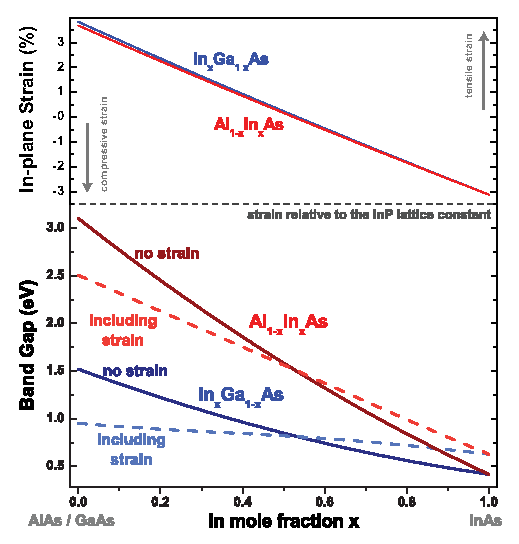
\includegraphics[width=4.5in]{chpt1_comp_panel}
\caption[Bandgap strain dependence]{\tn{\textbf{Bandgap strain dependence.}}  The top panel shows in-plane strain $\varepsilon_{xx}$ relative to the InP lattice constant (at $300~\tn{K}$) for In$_x$Ga$_{1-x}$As and Al$_{1-x}$In$_{x}$As of mole fraction $x$.  The bottom panel compares the effect of strain on bandgap for the same materials compositions.  Bandgap calculations where strain is ignored---that is, bandgaps only dependent upon material compositions---are shown as solid lines.  (Here, $\EE_{\tn{C}-\tn{LH}}^\Gamma$ and $\EE_{\tn{C}-\tn{HH}}^\Gamma$ are degenerate when strain is zero.)  Calculations for $\EE_{\tn{C}-\tn{LH}}^\Gamma$ that apply a correction for in-plane strain are shown as dashed lines.  The correction $\delta\!\EE_\tn{\textit{Varsh}}$ is not included here.}
\label{chpt1:strain_effect}
\end{figure}


\section{Effective Mass}

Just as important as the potential profile $V(z)$ to accurate solutions of the Schr\"{o}dinger equation is the effective mass.  Fundamentally, the effective mass of an individual energy band is influenced by the surrounding energy bands. Using $\textbf{k}\bullet \textbf{p}$ theory, the conduction band effective mass perpendicular to the plane of epitaxial growth $m^*\left(z,\EE_q\right)$ can be derived as \cite{Vurgaftman}, \cite{Sugawara:PRB:1993}, \cite{Sirtori:PRB:1994}
\begin{equation}
\label{chpt1eqn:effective_mass}
\frac{1}{m^*\left(z,\EE_q\right)} = \frac{1}{m_0} \left\{1+2F+\frac{\EE_P}{3} \left[ \frac{ \left(\sqrt{2} u-v\right)^2}{\EE_q + \EE_{\tn{C}-\tn{LH}}^\Gamma} + \frac{ \left(\sqrt{2} v+u \right)^2}{\EE_q + \EE_{\tn{C}-\tn{SO}}^\Gamma} \right] \right\}
\end{equation}
where each of the terms $F$, $\EE_P$, $u$, $v$, $\EE_q$, $\EE_{\tn{C}-\tn{LH}}^\Gamma$, and $\EE_{\tn{C}-\tn{SO}}^\Gamma$ have $z$-dependence.  The free space electron mass is $m_0$, $F$ is the Kane parameter representing the second-order $\textbf{k}\bullet \textbf{p}$ perturbation term, $\EE_P$ is the energy-unit representation of the momentum matrix element between the $s$-like conduction bands and $p$-like valence bands, $\EE_q$ is the energy of the quantized energy state above or below the conduction band, and $u$ and $v$ represent the degree of mixing between LH and SO states and are give as
\begin{equation}
u = \frac{2\sqrt{2} |Q_\varepsilon|}{C} \qquad \text{and} \qquad
v = \frac{(A-B) |Q_\varepsilon|}{C Q_\varepsilon}
\end{equation}
with
\begin{equation}
A=\Delta_{\tn{SO}}+Q_\varepsilon \text{ ,} \quad
B=\sqrt{\Delta_{\tn{SO}}^2+2 \Delta_{\tn{SO}} Q_\varepsilon +9 Q_\varepsilon^2}\text{ ,}\quad \text{and} \quad
C=\sqrt{2 B (B-A)} \text{~.}
\end{equation}
In the case of no strain, $u=1$ and $v=0$.  Moreover, for in-plane strain values up to $\sim\!2$\%, $u\approx1$ and $v\approx0$ so
\begin{equation}
\label{chpt1eqn:effective_mass_simple}
\frac{1}{m^*\left(z,\EE_q\right)} = \frac{1}{m_0} \left\{ 1+2F+ \frac{\EE_P}{3} \left[ \frac{2}{\EE_q + \EE_{\tn{C}-\tn{LH}}^\Gamma} + \frac{1}{\EE_q + \EE_{\tn{C}-\tn{SO}}^\Gamma} \right] \right\}
\end{equation}
is a good approximation.  Both $\EE_P$ and $F$ are well-reviewed for III--V materials by Vurgaftman \emph{et al.} \cite{Vurgaftman}, and they are generally considered to be independent of strain and temperature.  Using Eq.~\eqref{chpt1eqn:effective_mass} or \eqref{chpt1eqn:effective_mass_simple}, the energy dependence of the effective mass in a quantum well (\emph{i.e.} non-parabolicity) \cite{Sirtori:PRB:1994}, \cite{Nelson:PRB:1987} is taken into account by virtue of $\EE_q$.  Also, the effects of strain and temperature on effective mass are accounted for by their effects on the bandgaps $\EE_{\tn{C}-\tn{LH}}^\Gamma$ and $\EE_{\tn{C}-\tn{SO}}^\Gamma$.



\section[Self-consistent Solutions of the Schr\"{o}dinger and Poisson Equations]{Self-consistent Solutions of the Schr\"{o}dinger and \\ Poisson Equations}

Knowing the energy gaps and band offsets of our materials system, we can calculate the semiconductor material potential profile $V_{mat}(z)$. However, when semiconductors are doped, the fixed and free charges (ionized impurities and free electrons, respectively) that make up a charge distribution $\rho$ add a perturbation to the potential profile.  Given by the Poisson equation, this perturbation $V_\rho$ is
\begin{equation}
\nabla^2 V_\rho = -\frac{\rho}{\epsilon}
\end{equation}
where $\epsilon = \epsilon_r \epsilon_0$ is the material permittivity.  The potential $V_\rho(z)$ can otherwise be found through the electric field strength $E(z)$:
\begin{equation}
V_\rho(z)=\int_{-\infty}^z\!E(z)\,dz \tn{~.}
\end{equation}
With our system of energy states quantized in one dimension ($z$), and our wavefunctions $\psi(z)$ numerically solved at discrete points with spacing $\delta\!z$, we can think of the charge density $\rho(z)$ as infinite sheets, with sheet density $\sigma(z)$ and thickness $\delta\!z$ (similar to the process outlined by Harrison \cite{Harrison}).  The resultant perpendicular electric field to an infinite plane of charge is
\begin{equation}
E = \frac{\sigma}{2 \epsilon}
\end{equation}
and we can thus sum the contributions to the aggregate electric field from all of the individual ``slices'' of $\delta\!z$ as
\begin{equation}
E(z) = - \sum_{z'=-\infty}^{z-\delta\!z} \frac{\sigma(z')}{2\epsilon} +  \sum_{z'=z}^{\infty} \frac{\sigma(z')}{2\epsilon}
\end{equation}
which accounts for the sign of the field being dependent on the location of the position $z$ relative to the position of the charge slice $z'$.  The sheet charge density $\sigma(z)$ includes both negative free electron charge and positive ionized impurity charge.  For a doping density profile $N_d(z)$ [$\frac{1}{\tn{volume}}$], the total free electron sheet density $n_s$ [$\frac{1}{\tn{area}}$] will be given by
\begin{equation}
n_s = \int_{-\infty}^{+\infty} \! N_d(z) \, dz
\end{equation}
and the fixed charge sheet density is $N_d(z) \delta\!z$.  The net sheet charge density is thus
\begin{equation}
\sigma(z) = q \left[N_d(z) \delta\!z - n_s \psi_i^*(z) \psi_i(z) \right]
\end{equation}
where $q$ is the absolute value of the electron charge ($q=|q|$) and if all free electrons are in the quantum state $i$.  If all electrons are not in a single quantum state (\emph{i.e.} $T\neq0$~K), we can distribute them over the set of relevant states using the Fermi distribution as a weighting function.  For the quantum state $i$ at energy $\EE_i$, the Fermi distribution is
\begin{equation}
f(\EE_i) = \frac{1}{e^{\frac{(\EE_i-\EE_0)-\EE_\tn{F}(T)}{k_\tn{B} T}}+1}
\end{equation}
where $\EE_0$ is the energy of the lowest state in the QC period (the injector ground state, for example) and $\EE_\tn{F}(T)$ is the Fermi energy at temperature $T$ given by \cite{Davies:book:1998}
\begin{equation}
\EE_\tn{F}(T)=k_\tn{B} T \ln\left(e^{\frac{\EE_\tn{F}(0)}{k_\tn{B} T}}-1\right)
\end{equation}
and
\begin{equation}
\EE_\tn{F}(0)=n_s \frac{\pi \hslash^2}{m^*} \text{~.}
\end{equation}
Now, for $n_s$ electrons thermally distributed over quantum states 1 through $n$, the population in state $i$ can be determined by the weighting coefficient $\xi_i$ such that
\begin{equation}
\xi_i = \frac{f(\EE_i)}{\sum_{i=1}^{n} f(\EE_i)}
\end{equation}
and
\begin{equation}
n_i=\xi_i n_s
\end{equation}
so long as we ensure that the individual weighting coefficients sum to one $\left(\sum_{i=1}^{n} \xi_i = 1\right)$.
%\begin{equation}
%n_j=\frac{m k_\tn{B} T}{\pi \hslash^2} \ln \left[1+ e^{\frac{\EE-\EE_\tn{F}(T)}{k_\tn{B} T}}\right]
%\end{equation}
Our sheet charge density now becomes
\begin{equation}
\sigma(z) = q \left[N_d(z) \delta\!z - \sum_{i=1}^{n} \xi_i n_s \psi_i^*(z) \psi_i(z) \right]
\end{equation}
for the electron-occupied set of quantum states 1 through $n$.

Following the above procedure to find the charge potential $V_\rho$, we can apply this correction as a perturbation to the overall potential: $V(z)=V_{mat}(z)+V_\rho(z)$.  We can then solve our system using Eq.~\eqref{chpt1eqn:numerical_S_eq} and the shooting method described previously with the new composite potential.  Certainly, the perturbation from $V_\rho$ changes the solution to the system enough that a new $V_\rho$ can be calculated based on the shifted electron wavefunctions.  Thus, an iterative approach is needed, where $V_\rho$ is updated after each iteration until consecutive solutions converge.

%\beqin{subequations}
%\begin{gather}
%\sigma(z)=q \left( \sum_{i=1}{n} N_i \psi_i^*(z) \psi_i(z)-d(z) \right) \delta\!z\\
%\sigma(z) = q \right[ N \psi_i^*(z) \psi_i(z)-d(z) \right] \delta\!z\\
%\sum_{z=-\infty}{\infty}\sigma(z)=0 \text{   charge neutrality}\\
%\end{gather}
%\end{subequations}


\section{Spontaneous Emission Rate and the Optical Dipole Matrix Element}

The optical transition rate $W_\textit{opt}$ between two eigen states of a system, such as an upper state $\psi_\tn{\tiny{C}}^u$ and lower state $\psi_\tn{\tiny{C}}^\ell$, is given by first order perturbation theory (Fermi's golden rule) as \cite{CohenTannoudji}
\begin{equation}
\label{chpt1eqn:fermi_golden_rule1}
W_\textit{opt}^{\vec{k},\vartheta} = \frac{2 \pi}{\hslash} \vert\langle \psi_\tn{\tiny{C}}^\ell,\mathcal{N}^\ell_{\vec{k},\vartheta} \vert \mathscr{H}'\vert \psi_\tn{\tiny{C}}^u,\mathcal{N}^u_{\vec{k},\vartheta}  \rangle\vert^2 \delta(\EE_u-\EE_\ell-\EE_{\vec{k}})
\end{equation}
for the optical mode with wavevector $\vec{k}$ and polarization $\vartheta$,
where the interaction Hamiltonian $\mathscr{H}'$ is the light--matter perturbation responsible for the transition and the terms $\mathcal{N}^u_{\vec{k},\vartheta}$ and $\mathcal{N}^\ell_{\vec{k},\vartheta}$ represent quantized states (number of photons) of the electromagnetic field. % to the free electron Hamiltonian $\mathscr{H}_0$.
%is given by \cite{Yariv:book:1989}
%\begin{equation}
%\mathscr{H}' = -q \mathbf{E}_l (\mathbf{r},t) \cdot \mathbf{r}
%\end{equation}
The total Hamiltonian that includes light--matter interaction for an electron in the conduction band is given as \cite{CohenTannoudji}
\begin{equation}
\label{chpt1eqn:long-hamiltonian1}
\mathscr{H}=\frac{\left(\vec{\mathcal{P}}-q \textit{\textbf{A}}\right)^2}{2 m^*} + q V_\tn{\tiny{C}}(\vec{r})
\end{equation}
where $\vec{\mathcal{P}}$ is the momentum operator in three dimensions, $\vec{r}$ is a position vector, and assuming for the moment a constant effective mass $m^*$.
Taking $\textit{\textbf{A}}$ to be the vector potential of the optical field in the Coulomb gauge so that $\nabla\cdot \textit{\textbf{A}}=0$, Eq.~\eqref{chpt1eqn:long-hamiltonian1} becomes
\begin{equation}
\label{chpt1eqn:long-hamiltonian2}
\mathscr{H} = \frac{\vec{\mathcal{P}}^2}{2 m^*} -\frac{q}{m^*}\left(\textbf{\textit{A}} \cdot \vec{\mathcal{P}} \right) + \frac{q^2}{2 m^*} A^2 + q V_\tn{\tiny{C}}(\vec{r})
\end{equation}
after also using the commutation $[\vec{\mathcal{P}},\textit{\textbf{A}}]=0$ for the Coulomb gauge \cite{CohenTannoudji}.  We may assume that the term in $A^2$ is negligible given sufficiently small optical field intensity and matrix elements of $\vec{\mathcal{P}}$ \cite{Yariv:book:1989}; that is, we ignore two photon processes \cite{Parker:book:2005}.  Thus, our interaction Hamiltonian $\mathscr{H}'$ is
\begin{equation}
\label{chpt1eqn:Hprime}
\mathscr{H}'=-\frac{q}{m^*}\left(\textit{\textbf{A}} \cdot \vec{\mathcal{P}} \right)
\end{equation}
given that the remainder of Eq.~\eqref{chpt1eqn:long-hamiltonian2} is the unperturbed Hamiltonian
\begin{equation}
\mathscr{H}_0=\frac{\vec{\mathcal{P}}^2}{2 m^*} + q V_\tn{\tiny{C}}(\vec{r}) \tn{~.}
\end{equation}
Applying Eq.~\eqref{chpt1eqn:Hprime} to Eq.~\eqref{chpt1eqn:fermi_golden_rule1}, the optical transition rate is
\begin{equation}
\label{chpt1eqn:fermi_golden_rule2}
W_\textit{opt}^{\vec{k},\vartheta} = \frac{2 \pi}{\hslash} \frac{q^2}{m^{*2}} \vert\langle \psi_\tn{\tiny{C}}^\ell,\mathcal{N}^\ell_{\vec{k},\vartheta} \vert \textit{\textbf{A}} \cdot \vec{\mathcal{P}}
\vert \psi_\tn{\tiny{C}}^u,\mathcal{N}^u_{\vec{k},\vartheta}  \rangle\vert^2 \delta(\EE_u-\EE_\ell-\EE_{\vec{k}}) \tn{~.}
\end{equation}
The operator form of the vector potential $\textit{\textbf{A}}$ is derived using a plane wave expansion for a cavity with mode volume $\mathcal{V}_{\vec{k}}$ and permittivity $\epsilon$ as \cite{Parker:book:2005}
\begin{equation}
\textit{\textbf{A}}(\vec{r})=\sum_{\vec{k},\vartheta} \sqrt{\frac{\hslash}{2 \epsilon \omega_{\vec{k}} \mathcal{V}_{\vec{k}}}} \left[ \hat{b}^\dagger_{\vec{k},\vartheta} e^{-i \vec{k} \cdot \vec{r}} +  \hat{b}_{\vec{k},\vartheta} e^{i \vec{k} \cdot \vec{r}}\right]
\hat{e}_{\vec{k},\vartheta}
\end{equation}
where $\hat{e}_{\vec{k},\vartheta}$ is the unit vector for the photon mode, $\hat{b}^\dagger_{\vec{k},\vartheta}$ and $\hat{b}_{\vec{k},\vartheta}$ are the photon creation and annihilation operators, and the term $\sqrt{\frac{\hslash}{2 \epsilon \omega_{\vec{k}}}}$ provides MKS units.  We now invoke the dipole approximation, which treats the photon wavelength as being large compared to the space over which the optical transition occurs \cite{Parker:book:2005}. One result of the dipole approximation---with $|\vec{k}|=\frac{2\pi}{\lambda}\approx10^6$~m\sup{-1} and the electron confinement space in the QC active region $|\vec{r}|\approx10^{-8}$~m---is that $e^{i \vec{k} \cdot \vec{r}}\approx1$.  Also, using the relation $\mathcal{N}_{\vec{k},\vartheta}^\ell=\mathcal{N}_{\vec{k},\vartheta}^u+1$ since a photon is created in the transition \trans{\psi_\tn{\tiny{C}}^u}{\psi_\tn{\tiny{C}}^\ell},
\begin{subequations}
\begin{gather}
\langle \mathcal{N}_{\vec{k},\vartheta}^u+1 | \hat{b}^\dagger_{\vec{k},\vartheta} | \mathcal{N}_{\vec{k},\vartheta}^u \rangle =  \sqrt{\mathcal{N}_{\vec{k},\vartheta}^u+1} \langle \mathcal{N}_{\vec{k},\vartheta}^u+1 | \mathcal{N}_{\vec{k},\vartheta}^u+1 \rangle = \sqrt{\mathcal{N}_{\vec{k},\vartheta}^u+1}\\
\intertext{and}
\langle \mathcal{N}_{\vec{k},\vartheta}^u+1 | \hat{b}_{\vec{k},\vartheta} | \mathcal{N}_{\vec{k},\vartheta}^u \rangle = \sqrt{\mathcal{N}_{\vec{k},\vartheta}^u} \langle \mathcal{N}_{\vec{k},\vartheta}^u+1 | \mathcal{N}_{\vec{k},\vartheta}^u-1 \rangle = 0 \tn{~.}
\end{gather}
\end{subequations}
Finally, we can make the approximation that $\vec{\mathcal{P}}$ affects only the electron momentum, which is accurate in our low photon field approximation.  In this case, $\textit{\textbf{A}} \cdot \vec{\mathcal{P}}$ is separable so that $\langle \psi_\tn{\tiny{C}}^\ell | \vec{\mathcal{P}} | \psi_\tn{\tiny{C}}^u \rangle \cdot \langle \mathcal{N}_{\vec{k},\vartheta}^\ell \vert \textit{\textbf{A}} \vert \mathcal{N}_{\vec{k},\vartheta}^u  \rangle$
and Eq.~\eqref{chpt1eqn:fermi_golden_rule2} becomes
\begin{equation}
\label{chpt1eqn:fermi_golden_rule3}
W_\textit{opt}^{\vec{k},\vartheta} = \frac{\pi q^2}{\epsilon m^{*2} \mathcal{V}_{\vec{k}}}
\frac{\left(\mathcal{N}_{\vec{k},\vartheta}^u+1\right)}{\omega_{\vec{k}}}
\vert \hat{e}_{\vec{k},\vartheta} \cdot \langle \psi_\tn{\tiny{C}}^\ell \vert \vec{\mathcal{P}}
\vert \psi_\tn{\tiny{C}}^u\rangle\vert^2 \delta(\EE_u-\EE_\ell-\EE_{\vec{k}})
\end{equation}
for a single optical mode.  Now, by applying the commutation relation \cite{CohenTannoudji}
\begin{equation}
\vec{\mathcal{P}} = \frac{i m^*}{\hslash} [\mathscr{H}_0,\vec{r}]
\end{equation}
we get
\begin{equation}
\langle \psi_\tn{\tiny{C}}^\ell \vert \vec{\mathcal{P}}
\vert \psi_\tn{\tiny{C}}^u\rangle = \frac{i m^*}{\hslash} \langle \psi_\tn{\tiny{C}}^\ell \vert \mathscr{H}_0\cdot\vec{r} - \vec{r}\cdot\mathscr{H}_0 \vert \psi_\tn{\tiny{C}}^u\rangle = i m^* \omega_{0} \langle \psi_\tn{\tiny{C}}^\ell \vert \vec{r} \vert \psi_\tn{\tiny{C}}^u\rangle
\end{equation}
and so
\begin{equation}
W_\textit{opt}^{\vec{k},\vartheta} = \frac{\pi q^2}{\epsilon \mathcal{V}_{\vec{k}}} \left(\mathcal{N}_{\vec{k},\vartheta}^u+1\right) \omega_{0}
\vert\hat{e}_{\vec{k},\vartheta} \cdot \langle \psi_\tn{\tiny{C}}^\ell \vert \vec{r} \vert \psi_\tn{\tiny{C}}^u\rangle\vert^2 \delta(\EE_u-\EE_\ell-\EE_{\vec{k}}) \tn{~.}
\end{equation}
From here, we can separate two contributions to the optical transition rate: those of stimulated emission $W_\textit{stim}^{\vec{k},\vartheta}$ due to the presence of an inducing field proportional to $\mathcal{N}_{\vec{k},\vartheta}^u$ and spontaneous emission $W_\textit{spon}^{\vec{k},\vartheta}$ due to zero-point field such that
\begin{equation}
W_\textit{opt}^{\vec{k},\vartheta} = W_\textit{stim}^{\vec{k},\vartheta}+W_\textit{spon}^{\vec{k},\vartheta} \tn{~.}
\end{equation}
Since the wavefunctions $\psi_\tn{\tiny{C}}^u$ and $\psi_\tn{\tiny{C}}^\ell$ have quantization only in the $z$ direction, we can further simplify to
\begin{subequations}
\begin{gather}
W_\textit{stim}^{\vec{k},\vartheta} = \frac{\pi q^2}{\hslash \epsilon \mathcal{V}_{\vec{k}}} \omega_{0}
z_{u\ell}^2
|\hat{e}_{\vec{k},\vartheta} \cdot \hat{z} |^2  %\delta_{\vec{\kappa_{//}}^u,\vec{\kappa_{//}}^\ell}
\delta(\omega_0-\omega_{\vec{k}}) \mathcal{N}_{\vec{k},\vartheta}^u\\
W_\textit{spon}^{\vec{k},\vartheta} = \frac{\pi q^2}{\hslash \epsilon \mathcal{V}_{\vec{k}}} \omega_{0}
z_{u\ell}^2
|\hat{e}_{\vec{k},\vartheta} \cdot \hat{z} |^2  %\delta_{\vec{\kappa_{//}}^u,\vec{\kappa_{//}}^\ell}
\delta(\omega_0-\omega_{\vec{k}})
\label{chpt1eqn:WsponMode1}
\end{gather}
\end{subequations}
where $\hat{z}$ is the unit vector in the $z$ direction, the optical dipole matrix element $z_{u\ell}$ is defined as
\begin{equation}
z_{u\ell}\equiv\langle \psi_\tn{\tiny{C}}^\ell \vert z \vert \psi_\tn{\tiny{C}}^u\rangle
\end{equation}
and the transformation $\EE_u-\EE_\ell=\hslash \omega_0$ has been used.

Concentrating now just on the spontaneous emission, the total spontaneous emission rate is realized by summing over all modes in the optical cavity.  Equivalently, we can integrate over the product of all possible modes and the density of the cavity photon modes $\mathscr{D}$.
\begin{equation}
\label{chpt1eqn:WsponSum}
W_\textit{spon}=\sum_{\vec{k},\vartheta} W_\textit{spon}^{\vec{k},\vartheta} = \int \! \int \!\int W_\textit{spon}^{\vec{k},\vartheta} \times \mathscr{D}(\omega_{\vec{k}}) \, d^3 \omega_{\vec{k}}
\end{equation}
For an arbitrarily shaped electromagnetic enclosure where the dimensions are at least a few times the transition wavelength \cite{Smet:JAP:1996}, the differential mode density $\mathscr{D}_\tn{3D}(\omega_{\vec{k}}) d^3\omega_{\vec{k}}$ is given in spherical coordinates as \cite{SalehTeich:book:1991}% and the term $\delta_{\vec{\kappa_{//}}^u,\vec{\kappa_{//}}^\ell} $ ensures conservation of the in-plane electron wavevector $\vec{\kappa_{//}}$.
\begin{equation}
\label{chpt1eqn:photonD3D}
\mathscr{D}_\tn{3D}(\omega_{\vec{k}}) d^3\omega_{\vec{k}} = \frac{d^3\omega_{\vec{k}}}{\frac{8 \pi^3}{\mathcal{V}_{\vec{k}}}} = \frac{\mathcal{V}_{\vec{k}}}{8 \pi^3} \, k^2 \sin \theta \, d\vec{k} \, d\theta \, d\phi = \frac{n_\textit{eff}^3}{c_0^3} \frac{\mathcal{V}_{\vec{k}}}{8 \pi^3} \omega_{\vec{k}}^2 \sin\theta \, d\omega_{\vec{k}} \, d\theta \, d\phi
\end{equation}
where $n_\textit{eff}$ is the effective refractive index of the mode, $c_0$ is the speed of light in vacuum, $\theta$ is the zenith angle from the positive $z$-axis, and $\phi$ is the azimuth angle from the positive $x$-axis. Combining Eqs.~\eqref{chpt1eqn:WsponMode1} and \eqref{chpt1eqn:photonD3D} into Eq.~\eqref{chpt1eqn:WsponSum} gives
\begin{equation}
W_\textit{spon}=\frac{q^2 n_\textit{eff}^3 \;\omega_0}{8 \pi^2 \hslash \epsilon c_0^3} z_{u\ell}^2 \int_0^\infty \omega_{\vec{k}}^2 \delta(\omega_0 - \omega_{\vec{k}}) d\omega_{\vec{k}} \int_0^{2\pi}\!\int_0^{\pi}|\hat{e}_{\vec{k},\vartheta} \cdot \hat{z}|^2 \sin \theta d\theta d\phi \tn{~.}
\end{equation}
For the two orthogonal polarizations $\hat{e}_{\vec{k},\vartheta=1}$ and $\hat{e}_{\vec{k},\vartheta=2}$, we can choose $\hat{e}_{\vec{k},\vartheta=1}$ to lie in the plane of $\hat{z}$ and $k_z$ so that $|\hat{e}_{\vec{k},\vartheta=2}\cdot \hat{z}|^2=0$.  Using $|\hat{e}_{\vec{k},\vartheta} \cdot \hat{z}|^2=\sin^2\theta$ and $\epsilon=n_\textit{eff}^2 \epsilon_0$, the spontaneous emission rate is \cite{Yariv:book:1989} \cite{Parker:book:2005} \cite{Smet:JAP:1996}  \cite{Rosencher:book:2002}
\begin{equation}
\label{chpt1eqn:tspon}
W_\textit{spon}=\frac{1}{\tau_\textit{spon}}=\frac{q^2 n_\textit{eff} \: \omega_0^3}{3 \pi \hslash \epsilon_0 c_0^3} z_{u\ell}^2
\end{equation}
where $\tau_\textit{spon}$ is the spontaneous emission lifetime.
%We can now separate the two contributions to the optical transition rate, those of stimulated emission $W_\textit{stim}$ and spontaneous emission $W_\textit{spon}$
%\begin{subequations}
%\begin{gather}
%W_\textit{stim}=\frac{q^2 n_\textit{eff} \: \omega_0^3}{3 \pi \hslash \epsilon_0 c_0^3} z_{u\ell}^2 \mathcal{N}_{ph}\\
%W_\textit{spon}=\frac{q^2 n_\textit{eff} \: \omega_0^3}{3 \pi \hslash \epsilon_0 c_0^3} z_{u\ell}^2
%\end{gather}
%\end{subequations}

\subsubsection{Normalization of the wavefunctions $\mathbf{\psi}_\tn{\tiny{\tb{C}}}$}

To this point in our derivation of $\tau_\textit{spon}$, we have assumed an effective mass $m^*$ that is constant with energy.  We now appropriately account for the variable effective mass with proper normalization the wavefunctions $\psi_\tn{\tiny{C}}$ that are used to calculate our optical dipole matrix element $z_{u\ell}$.

In previous sections, our solutions for conduction band eigenstates $\psi_\tn{\tiny{C}}$ have used the envelope function Hamiltonian in the Kane approximation \cite{Bastard:book:1991}.  In the Kane approximation, the full system Hamiltonian is projected onto the individual subbands (conduction band, light hole band, etc.).  If the in-plane electron momentum is assumed to vanish, the total stationary wavefunction is given by the three components $\psi_\tn{\tiny{C}}$, $\psi_\tn{\tiny{LH}}$, and $\psi_\tn{\tiny{SO}}$, weighted with their corresponding Bloch functions \cite{Sirtori:PRB:1994}.  Consequently, knowledge of only the conduction component $\psi_\tn{\tiny{C}}$ is insufficient for the complete physical description of the stationary state, and the stationary state is thus normalized as \cite{Sirtori:PRB:1994}
\begin{equation}
\label{chpt1eqn:norm1}
\langle \psi_\tn{\tiny{C}} | \psi_\tn{\tiny{C}} \rangle + \langle \psi_\tn{\tiny{LH}} | \psi_\tn{\tiny{LH}} \rangle + \langle \psi_\tn{\tiny{SO}} | \psi_\tn{\tiny{SO}} \rangle = 1
\end{equation}
However, just as our calculation of the energy-dependent effective mass in Eq.~\eqref{chpt1eqn:effective_mass} included the conduction band interaction with the valence bands, we can likewise recast Eq.~\eqref{chpt1eqn:norm1} entirely in terms of $\psi_\tn{\tiny{C}}$ as \cite{Sirtori:PRB:1994}
\begin{equation}
\label{chpt1eqn:norm2}
\langle \psi_\tn{\tiny{C}} | 1+\frac{2}{3}\mathcal{P}_z \frac{\EE_P}{2 m_0 \left(\EE_q+\EE_{\tn{LH}}^\Gamma\right)^2} \mathcal{P}_z +  \frac{1}{3}\mathcal{P}_z \frac{\EE_P}{2 m_0 \left(\EE_q+\EE_{\tn{SO}}^\Gamma\right)^2} \mathcal{P}_z| \psi_\tn{\tiny{C}} \rangle= 1 \tn{~.}
\end{equation}
Defining the average valence band energy as
$\EE_v = \frac{2 \EE_\tn{LH} + \EE_\tn{SO}}{3}$, we may further simplify Eq.~\eqref{chpt1eqn:norm2} and approximate it as \cite{Leavitt:PRB:1991}
\begin{equation}
\langle \psi_\tn{\tiny{C}} |1 + \frac{\mathcal{P}_z^2}{2 m^*(\EE_q) (\EE_q+\EE_v)} | \psi_\tn{\tiny{C}} \rangle = 1
\end{equation}
or equivalently
\begin{equation}
\langle \psi_\tn{\tiny{C}} |1 +  \frac{\EE_q}{\EE_q+\EE_v} | \psi_\tn{\tiny{C}} \rangle = 1 \tn{~.}
\end{equation}


%The optical dipole matrix element $z_{u\ell}$ between an initial (upper) state $u$ and final (lower) state $\ell$ is $\langle \psi_u^C | z | \psi_\ell^C \rangle$.  The values of $\psi^C$ must be properly normalized.


\section{Stimulated Emission Probability and the Transition Cross Section}
In the previous section, we derived the probability of stimulated emission for a single optical mode $\vec{k}$ as
\begin{equation}
W_\textit{stim}^{\vec{k},\vartheta} = \frac{\pi q^2}{\hslash \epsilon \mathcal{V}_{\vec{k}}} \omega_{\vec{k}}
z_{u\ell}^2
|\hat{e}_{\vec{k},\vartheta} \cdot \hat{z} |^2  \delta(\omega_0-\omega_{\vec{k}}) \mathcal{N}_{\vec{k},\vartheta}^u
\end{equation}
In general, the transition frequency $\omega_0$ is not a single value, but is instead broadened.  We thus substitute $\delta(\omega_0-\omega_{\vec{k}})$ for the normalized Lorentzian lineshape function $\mathscr{L}(\nu)$ given as
\begin{equation}
\mathscr{L}(\nu)=\frac{\frac{\delta\!\nu}{2\pi}}{(\nu_0-\nu)^2+\left(\frac{\delta\!\nu}{2} \right)^2} %\quad \text{and} \quad
%\mathscr{L}(\omega)=\frac{\delta\!\omega}{(\omega_0-\omega)^2+\left(\frac{\delta\!\omega}{2} \right)^2}
\end{equation}
and then integrate over $\nu$.  Now, the stimulated emission probability becomes \cite{Yariv:book:1989}
\begin{equation}
W_\textit{stim}^{\vec{k},\vartheta}=\frac{\pi q^2 z_{u\ell}^2 \mathcal{N}_{\vec{k},\vartheta}}{h \mathcal{V}_{\vec{k}} \epsilon} \mathscr{L}(\nu)
\end{equation}
We can also now relate the number of mode photons $\mathcal{N}_{\vec{k},\vartheta}$ to a photon mode flux $\phi_{ph}$ $[\frac{\tn{photons}}{\tn{area}\times\tn{time}}]$ using the group velocity $v_g$ where
\begin{equation}
\phi_{ph} = \frac{v_g}{\mathcal{V}_{\vec{k}}} \mathcal{N}_{\vec{k},\vartheta}
\end{equation}
so that \cite{Yariv:book:1989}
\begin{equation}
W_\textit{stim} = \phi_{ph} \frac{3 \lambda_0^2}{8 \pi \tau_\textit{spon}} \mathscr{L}(\nu)
\end{equation}
where Eq.~\eqref{chpt1eqn:tspon} is used to eliminate $z_{u\ell}^2$.  The factor of 3 results from the polarization of the cavity mode \cite{Siegman:book:1986}.  Now, a useful quantity known as the transition cross section $\sigma(\nu)~[\small{\tn{area}}]$ and defined as \cite{SalehTeich:book:1991}
\begin{equation}
W_\textit{stim}=\phi_{ph} \sigma(\nu)
\end{equation}
is given by
\begin{equation}
\sigma(\nu) = \frac{2 \pi^2 q^2 \EE_{ph}}{h^2 c \epsilon_0 n_\textit{eff}} z_{u\ell}^2 \mathscr{L}(\nu)
\end{equation}
and $\sigma(\nu_0)=\sigma_0$ where $\nu_0$ is the lasing frequency at the photon energy $\EE_{ph}$ is
\begin{equation}
\sigma_0 = \frac{4 \pi q^2}{h c \epsilon_0 n_\textit{eff}} \frac{\EE_{ph}}{\delta\!\EE_{u\ell}} z_{u\ell}^2 \tn{~.}
\end{equation}

%
%\begin{equation}
%\mathscr{L}(\nu)=\frac{\frac{\delta\!\nu}{2\pi}}{(\nu_0-\nu)^2+\left(\frac{\delta\!\nu}{2} \right)^2} \quad \text{and} \quad
%\mathscr{L}(\omega)=\frac{\delta\!\omega}{(\omega_0-\omega)^2+\left(\frac{\delta\!\omega}{2} \right)^2}
%\end{equation}
%
%\begin{equation}
%P=\frac{1}{2} \epsilon_0 n c E_0^2
%\end{equation}

%A useful quantity in laser devices is the transition $\sigma(\nu)$ cross-section, defined in the relation \cite{SalehTeich:book:1991}
%\begin{equation}
%W_\textit{spon} = c \int_{0}^\infty \sigma(\nu) \mathscr{D}(\nu) d\nu
%\end{equation}
%where $\mathscr{D}(\nu)=\frac{8 \pi \nu^2}{c^3}$.  As a
%
%Taking now our relationship between rates of spontaneous and stimulated emission,
%\begin{equation}
%W_\textit{stim} = W_\textit{spon} \mathcal{N}_{ph}
%\end{equation}


\section{LO-phonon Scattering Time}
The fastest scattering process between energy states within the same band of semiconductor quantum wells is the non-radiative longitudinal optical (LO) phonon transition \cite{Ferreira:PRB:1989}.  Because it is the fastest transition process, quantifying the LO phonon lifetime becomes particularly relevant for QC laser design.  Charge carrier interaction with the electric polarization produced by the relative displacement of the positive and negative ions of polar semiconductors is referred to as the Fr\"{o}hlich interaction.  The Fr\"{o}hlich Hamiltonian $\mathscr{H}_F$ is given as
\begin{equation}
\mathscr{H}_F = \sum_{\mathbf{Q}} \sqrt{\frac{2 \pi \hslash\omega_\tn{LO} q^2}{(\epsilon_\infty - \epsilon_s) \mathcal{V}_Q Q^2}} e^{-i \mathbf{Q}\cdot\mathbf{r}} a_\mathbf{Q}^\dag
\end{equation}
where $\hslash\omega_{\tn{LO}}$ is the LO phonon energy, $\epsilon_\infty$ is the high frequency relative permittivity, $\epsilon_s$ is the static relative permittivity, $\mathcal{V}_Q$ is the volume of the system, $Q$ is the magnitude of the phonon wavevector $\mathbf{Q}$, $\mathbf{r}$ is the position vector, and $a_\mathbf{Q}^\dag$ is the creation operator for a phonon in the mode $\mathbf{Q}$.  Using Fermi's golden rule, the LO phonon lifetime $\tau_{u\ell}$ between an initial (upper) state $|u,\mathbf{k}_u\rangle$ and final (lower) state $|\ell,\mathbf{k}_\ell\rangle$ with electron wavevector $\mathbf{k}$ at $T=0$~K is then
\begin{equation}
\label{chpt1eqn:tau_complicated}
\frac{1}{\tau_{u\ell}} = \frac{\sqrt{m^*\!\left(\EE_u\right) m^*\!\left(\EE_\ell\right)} q^2 \omega_{\tn{LO}}}{2 \hslash^2 (\epsilon_\infty - \epsilon_s)} \int\limits_0^{2 \pi} \frac{\int\limits_{-\infty}^{+\infty} \! \int\limits_{-\infty}^{+\infty} \! \psi_\tn{\tiny{C}}^u(z) \psi_\tn{\tiny{C}}^\ell (z) e^{-Q|z-z'|} \psi_\tn{\tiny{C}}^u(z') \psi_\tn{\tiny{C}}^\ell (z') \, dz \, dz'}{Q} \sin\theta d\theta
\end{equation}
where $Q$ is given by
\begin{equation}
Q=\sqrt{k_u^2+k_\ell^2-2 k_u k_\ell \cos\theta}
\end{equation}
and $k_u$ and $k_\ell$ are related by
\begin{equation}
k_\ell^2 = \frac{m^*\!\left(\EE_\ell\right)}{m^*\!\left(\EE_u\right)} k_u^2 + \frac{2 m^*\!\left(\EE_\ell\right)}{\hslash^2} \left(\EE_{u\ell}-\hslash\omega_{\tn{LO}}\right) \tn{~.}
\end{equation}
If we assume the electron initially starts at wavevector $k_u=0$, then
\begin{equation}
k_\ell = \sqrt{\frac{2 m^*\!\left(\EE_\ell\right)}{\hslash^2} \left(\EE_{u\ell}-\hslash\omega_{\tn{LO}}\right)}
\end{equation}
and $Q=k_\ell$ so Eq.~\eqref{chpt1eqn:tau_complicated} simplifies to
\begin{equation}
\frac{1}{\tau_{u\ell}} = \frac{\sqrt{m^*\!\left(\EE_u\right) m^*\!\left(\EE_\ell\right)} q^2 \omega_{\tn{LO}}}{2 \hslash^2 (\epsilon_\infty - \epsilon_s)} \int_{-\infty}^{+\infty} \! \int_{-\infty}^{+\infty} \!  \frac{\psi_\tn{\tiny{C}}^u(z) \psi_\tn{\tiny{C}}^\ell (z) e^{-k_\ell|z-z'|} \psi_\tn{\tiny{C}}^u(z') \psi_\tn{\tiny{C}}^\ell (z')}{k_\ell}  \, dz \, dz' \tn{~.}
\end{equation}

The temperature dependence of $\tau_{u\ell}$ is attained by modifying the $T=0$~K rate using the Bose--Einstein occupation number for phonons of energy $\hslash\omega_\tn{LO}$.  Specifically, taking into account both phonon emission and absorption processes \cite{Ferreira:PRB:1989},
\begin{equation}
\frac{1}{\tau_{u\ell}(T)} = \frac{1}{\tau_{u\ell}(0)}  \left(1 + \frac{2}{e^{\frac{\hslash\omega_\tn{LO}}{k_\tn{B} T}}-1} \right) \tn{~.}
\end{equation}


%\section{Figure of Merit and Modal Gain}


%\section{Forms of Optical Loss}
%
%\subsection{Free carrier absorption}
%
%\subsection{Intersubband resonant absorption}


\section{Threshold Current}

\begin{figure}[tp]
\centering
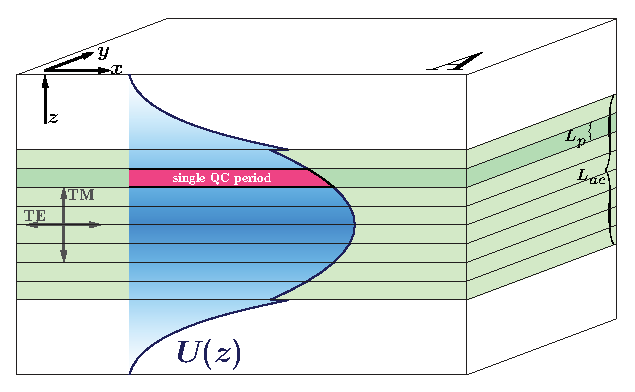
\includegraphics[width=4.5in]{waveguide_sketch}
\caption[Sketch of waveguide geometry]{\tn{\textbf{Sketch of waveguide geometry.}} A one dimensional optical mode profile (TM polarization) is shown as $U(z)$.  Multiple QC periods with higher refractive index than the surrounding cladding confine the mode, and the reduced field intensity for off-center QC periods is seen.  The arrows labeled TM and TE show direction of the electric field vector for the respective polarization.}
\label{chpt1:wg_sketch}
\end{figure}

Material gain $\gamma~[\frac{1}{\tn{length}}]$ is defined such that light intensity $\mathcal{I}$ after some distance $L$ is given by
\begin{equation}
\mathcal{I}(L) = \mathcal{I}(0) e^{\gamma L}
\end{equation}
and
\begin{equation}
\gamma = \begin{subarray}{c}\tn{gain region}\\\tn{overlap with}\\\tn{optical mode}\end{subarray} \times \begin{subarray}{c}\tn{``strength'' of the}\\\tn{gain material}\end{subarray}
\times \begin{subarray}{c}\tn{population}\\\tn{inversion}\end{subarray} = \Gamma \sigma_0 (N_u-N_\ell)
\end{equation}
where $(N_u-N_\ell)~[\frac{1}{\tn{volume}}]$ represents the population inversion density between the upper $u$ and lower $\ell$ states of the optical transition. The transition (gain) cross-section at peak gain $\sigma_0 \left[\tn{area}\right]$ as previously derived for the mode photon energy $\EE_{ph}$ is
\begin{equation}
\sigma_0 = \frac{4 \pi q^2}{h c \epsilon_0 n_\textit{eff}} \frac{\EE_{ph}}{\delta\!\EE_{u\ell}} z_{u\ell}^2
\end{equation}
and the one-dimensional confinement factor $\Gamma$ is defined as \cite{ColdrenCorzine}
\begin{equation}
\label{chpt1eqn:Gamma}
\Gamma = \frac{\int_{z_0}^{z_0+L_{ac}} \! U(z) \, dz}{\int_{-\infty}^{+\infty} \! U(z) \, dz}
\end{equation}
where $z_0$ marks the beginning of the active core, $L_{ac}$ is the thickness of the active core, %$n_r(z)$ is the refractive index profile, 
%and $f(z)$ is the electric field profile of the mode normalized such that $\max(f(z))=1$.
and $U(z)$ is the mode intensity profile normalized such that $\int U(z) dz=1$.  The confinement factor can then be used to identify an ``effective mode volume'' $\mathcal{V}_{ph}$ such that
\begin{equation}
\mathcal{V}_{ph}\equiv\frac{\mathcal{V}_{ac}}{\Gamma}
\end{equation}
where $\mathcal{V}_{ac}=A L_{ac}$ is the volume of the active core.  We now also have a 1D ``mode thickness'' $L_{ph}$ analogous to the active core thickness $L_{ac}$ given as
\begin{equation}
L_{ph}\equiv\frac{L_{ac}}{\Gamma}
\end{equation}
so that $\mathcal{V}_{ph}=A L_{ph}$.

further simplified by defining $L_m=\int_{-\infty}^{+\infty} \! n_r(z) f^2(z) \, dz$ as the effective thickness of the optical mode, and so the effective mode volume $\mathcal{V}_{ph}=A L_m$.

A QC laser adds the complication of multiple periods of the active--injector region structure cascaded together into a single active core.  In a general sense, each individual QC period $i$ may have its own unique properties.  Aggregate properties for the whole of the QC structure are given by summing over the individual QC periods.
\begin{equation}
\label{chpt1eqn:gamma_sum}
\gamma = \sum_{i=1}^{N_p} \Gamma_i \sigma_{0,i} (N_{u,i}-N_{\ell,i})
\end{equation}
where $\Gamma_i$ is now defined for an individual QC period as
\begin{equation}
\Gamma_i = \frac{\int_{z_i}^{z_i+L_{p}} \! n_r(z) f^2(z) \, dz}{L_m}
\end{equation}
with $L_{p}$ being the thickness of the QC active--injector period, so that summing over all $L_p$ yields $L_{ac}$ and summing over all $\Gamma_i$ yields the composite active core $\Gamma$.

Laser threshold is most easily derived assuming the gain clamping condition
\begin{equation}
\label{chpt1eqn:gain_clamp}
\gamma = \alpha_\textit{total}
\end{equation}
with total optical loss $\alpha_\textit{total}~[\frac{1}{\tn{length}}]$ being the sum of mirror loss $\alpha_m$ and waveguide loss $\alpha_w$.  Assuming each active period has the same transition cross-section and lifetime profile, applying Eq.~\eqref{chpt1eqn:gamma_sum} to Eq.~\eqref{chpt1eqn:gain_clamp} yields
\begin{equation}
\alpha_m + \alpha_w = N_p \Gamma \sigma_0 (N_{u}-N_{\ell})_\textit{th}
\end{equation}
where $N_p$ results from summing over all active periods and the population density $(N_{u}-N_{\ell})_\textit{th}$ is at threshold.  For a single QC period,
\begin{equation}
(N_{u,i}-N_{\ell,i})_\textit{th} = \begin{subarray}{c}\tn{pumping}\\\tn{rate}\end{subarray} \times \begin{subarray}{c}\tn{effective upper}\\\tn{state lifetime}\end{subarray}
= \frac{J_{th}}{q d_\textit{ap,i}} \tau_\textit{eff,i}
\end{equation}
where $\tau_\textit{eff}$ is the effective upper state lifetime.  For the case of a two level system at threshold (neglecting stimulated emission), $\tau_\textit{eff}=\tau_u \left(1-\frac{\tau_\ell}{\tau_{u\ell}}\right)$.  Thus,
\begin{equation}
J_{th} = q \frac{\alpha_\textit{total}}{ \Gamma \frac{N_p}{L_{ac}} \sigma_0 \tau_\textit{eff}} = \frac{h c \epsilon_0 n_\textit{eff}}{4 \pi q} \frac{\alpha_\textit{total}}{ \Gamma \frac{N_p}{L_{ac}} \frac{\EE_{u\ell}}{\delta\!\EE_{u\ell}} z_{u\ell}^2 \tau_\textit{eff} } \tn{~.}
\end{equation}

\section{Rate Equations for QC Lasers}
Rate equations are a phenomenological method for describing laser devices from which important performance parameters (\emph{e.g.}\ output power, wall-plug efficiency, threshold, etc.) can be derived.  Before directly discussing rate equations for QC lasers, it is important to recognize some of their unique properties.  These properties extend from the fact that QC lasers have multiple periods of gain region within the QC core, and each individual period can have its own local properties of photon field intensity and temperature; each period can furthermore have individually-customized emission \cite{Gmachl:2002:Nature:broadband} and doping profiles \cite{Hoffman:OptExp:2007} that can be treated accordingly by the rate equations. In the following discussion, we restrict ourselves to the case where the design of individual QC periods is identical.  In this case, we must concern ourselves only with the local field intensity and the local electron populations for each period.

In semiconductor lasers, field intensities in the gain region are usually treated through the use of confinement factor $\Gamma$, which is defined for the 1D case as \cite{ColdrenCorzine}
\begin{equation}
\label{chpt1eqn:Gamma}
\Gamma = \frac{\int_{z_0}^{z_0+L_{ac}} \! n_r(z) U(z) \, dz}{\int_{-\infty}^{+\infty} \! n_r(z) U(z) \, dz}
\end{equation}
where $z_0$ marks the beginning of the active core, $L_{ac}$ is the thickness of the active core, $n_r(z)$ is the refractive index profile,
and $U(z)$ is the dimensionless mode intensity profile normalized such that $\max(U(z))=1$.  The mode profile $U(z)$ can also be used to identify an ``effective mode volume'' $\mathcal{V}_{ph}$, here for the 1D case, such that
\begin{equation}
\mathcal{V}_{ph} = A \int_{-\infty}^{+\infty} \! U(z) \, dz
\end{equation}
where $A$ is the device area in the $x$ and $y$ dimensions, and so that the active core volume $\mathcal{V}_{ac}=A L_{ac}$.  We now also have a 1D ``mode thickness'' $L_{ph}$ analogous to the active core thickness $L_{ac}$ given as
\begin{equation}
L_{ph} = \int_{-\infty}^{+\infty} \! U(z) \, dz \tn{~.}
\end{equation}
In the typical set of rate equations describing diode lasers, which do not address the QC feature of a multiple gain region stack, it is commonly assumed that the gain profile is a square function over the active region, and so $\Gamma=\frac{L_{ac}}{L_{ph}}$; here, the refractive index profile $n_r(z)$ is also assumed to be constant.  We will not make these assumptions in the following rate equation analysis for QC structures.  Instead, we will use a ``local field coefficient'' $\bar{U}_i$ for an individual QC period $i$ given as 
\begin{equation}
\bar{U}_i = \frac{\int_{z_i}^{z_i+L_{p}} \! n_r(z) U(z) \, dz}{\int_{z_i}^{z_i+L_p} \! n_r(z) \, dz}
\end{equation}
where $z_i$ marks the beginning of the QC period.  If the active period thickness $L_p$ is sufficiently thin, $\bar{U}_i\approx U(z_i)$.

In QC structures, the local electron populations can be individually affected by such things as the local field intensity and the local temperature.  Thus, in the following analysis, we will treat the energy state populations of each QC period individually.  Describing the change with respect to time in the upper state population $\mathcal{N}_{u,i}$, lower state population $\mathcal{N}_{\ell,i}$, and \emph{total} photon population $\mathcal{N}_{ph}$ of the system gives the system of equations,
\begin{subequations}
%\setstretch{1.5}
\label{chpt1eqn:req_words}
\begin{align}
\mathcal{N}_{u,i}\: \begin{subarray} \tn{change}\\\tn{w.r.t. time}\end{subarray} &= \begin{subarray}{c}\tn{non-radiative}\\\tn{rate in}\end{subarray} - \begin{subarray}{c}\tn{non-radiative}\\\tn{rate out}\end{subarray} - \begin{subarray}{c}\tn{radiative}\\\tn{transition rate}\end{subarray}\\
\mathcal{N}_{\ell,i}\: \begin{subarray} \tn{change}\\\tn{w.r.t. time}\end{subarray} &= \begin{subarray}{c}\tn{non-radiative}\\\tn{rate in}\end{subarray} - \begin{subarray}{c}\tn{non-radiative}\\\tn{rate out}\end{subarray} + \begin{subarray}{c}\tn{radiative}\\\tn{transition rate}\end{subarray}\\
\mathcal{N}_{ph}\: \begin{subarray} \tn{change}\\\tn{w.r.t. time}\end{subarray} &= \begin{subarray}{c}\tn{sum over}\\\tn{all QC periods}\end{subarray} \left(\begin{subarray}{c}\tn{radiative}\\\tn{transition rate}\end{subarray}\right) - \begin{subarray}{c}\tn{photon}\\\tn{loss rate}\end{subarray}
\end{align}
\end{subequations}
where non-radiative transition rates are given by the population of the state $\mathcal{N}_{x,i}$ divided by the non-radiative lifetime $\tau_x$ for the energy state $x$.  Radiative transition rates are given by
\begin{gather*}
\begin{subarray}{c}\tn{radiative}\\\tn{transition rate}\end{subarray} =
\left( \begin{subarray}{c}\tn{population}\\\tn{available for}\\\tn{stimulated emission}\end{subarray} - \begin{subarray}{c}\tn{population}\\\tn{available for}\\\tn{absorption}\end{subarray}\right) \times \begin{subarray}{c}\tn{probability of}\\\tn{stimulated emission}\end{subarray}\\
\intertext{and}
\begin{subarray}{c}\tn{probability of}\\\tn{stimulated emission}\end{subarray} = \begin{subarray}{c}\tn{photon}\\\tn{density}\end{subarray} \times \begin{subarray}{c}\tn{photon}\\\tn{speed}\end{subarray} \times \begin{subarray}{c}\tn{transition}\\\tn{cross-section}\end{subarray} \times
\begin{subarray}{c}\tn{local field}\\\tn{strength of mode}\end{subarray} \tn{~.}
\end{gather*}
Now, making Eq.~\eqref{chpt1eqn:req_words} more explicit, our QC laser rate equations are thus generally expressed as
\begin{subequations}
\label{chpt1eqn:req1}
\begin{align}
\frac{d \mathcal{N}_{u,i}}{dt} &= \eta_\textit{inj}\frac{I}{q} - \frac{\mathcal{N}_{u,i}}{\tau_u} - \left( \mathcal{N}_{u,i} - \mathcal{N}_{\ell,i}\right) \frac{\mathcal{N}_{ph}}{\mathcal{V}_{ph}} v_g \sigma_i \bar{U}_i \\
%
\frac{d \mathcal{N}_{\ell,i}}{dt} &= \frac{\mathcal{N}_{u,i}}{\tau_{u\ell}} - \frac{\mathcal{N}_{\ell,i}}{\tau_\ell} + \left( \mathcal{N}_{u,i} - \mathcal{N}_{\ell,i}\right) \frac{\mathcal{N}_{ph}}{\mathcal{V}_{ph}} v_g \sigma_i \bar{U}_i\\
%
\frac{d \mathcal{N}_{ph}}{dt} &= \sum_{i=1}^{N_p}\left[ \left( \mathcal{N}_{u,i} - \mathcal{N}_{\ell,i}\right) \frac{\mathcal{N}_{ph}}{\mathcal{V}_{ph}} v_g \sigma_i \bar{U}_i \right] - \frac{\mathcal{N}_{ph}}{\tau_{ph}}
\end{align}
\end{subequations}
where $\eta_\textit{inj}\frac{I}{q}$ is the pumping rate for the upper laser state, $\tau_{ph}$ is the photon lifetime in the cavity, and $\sigma_i$ is the transition cross-section for the period $i$.  The group velocity $v_g$ is approximated by the phase velocity $c_0/n_\textit{eff}$, which is accurate when dispersion is low.










Describing the change with respect to time in the total upper state population $\mathcal{N}_u$, total lower state population $\mathcal{N}_\ell$, and total photon population $\mathcal{N}_{ph}$ of the system gives the system of equations,
\begin{subequations}
%\setstretch{1.5}
\begin{align}
\mathcal{N}_u\: \begin{subarray} \tn{change}\\\tn{w.r.t. time}\end{subarray} &= \begin{subarray}{c}\tn{non-radiative}\\\tn{rate in}\end{subarray} - \begin{subarray}{c}\tn{non-radiative}\\\tn{rate out}\end{subarray} - \begin{subarray}{c}\tn{radiative}\\\tn{transition rate}\end{subarray}\\
\mathcal{N}_\ell\: \begin{subarray} \tn{change}\\\tn{w.r.t. time}\end{subarray} &= \begin{subarray}{c}\tn{non-radiative}\\\tn{rate in}\end{subarray} - \begin{subarray}{c}\tn{non-radiative}\\\tn{rate out}\end{subarray} + \begin{subarray}{c}\tn{radiative}\\\tn{transition rate}\end{subarray}\\
\mathcal{N}_{ph}\: \begin{subarray} \tn{change}\\\tn{w.r.t. time}\end{subarray} &= \begin{subarray}{c}\tn{radiative}\\\tn{transition rate}\end{subarray} - \begin{subarray}{c}\tn{photon}\\\tn{loss rate}\end{subarray}
\end{align}
\end{subequations}
where non-radiative transition rates are given by the population of the state $\mathcal{N}_i$ divided by the non-radiative lifetime $\tau_i$ for the state $i$.  Radiative transition rates are given by
\begin{gather*}
\begin{subarray}{c}\tn{radiative}\\\tn{transition rate}\end{subarray} =
\left( \begin{subarray}{c}\tn{population available}\\\tn{for stimulated}\\\tn{emission}\end{subarray} - \begin{subarray}{c}\tn{population available}\\\tn{for absorption}\end{subarray}\right) \times \begin{subarray}{c}\tn{probability of}\\\tn{stimulated}\\\tn{emission}\end{subarray}\\
\intertext{and}
\begin{subarray}{c}\tn{probability of}\\\tn{stimulated}\\\tn{emission}\end{subarray} = \begin{subarray}{c}\tn{photon}\\\tn{density}\end{subarray} \times \begin{subarray}{c}\tn{photon}\\\tn{speed}\end{subarray} \times \begin{subarray}{c}\tn{transition}\\\tn{cross-section}\end{subarray} \times
\begin{subarray}{c}\tn{local field}\\\tn{strength of mode}\end{subarray} \tn{~.}
\end{gather*}
While many representations of rate equations assume the electric (\emph{i.e.} photon) field strength is homogenous over the gain region, this is not the case in the general sense.  Rather, both the field strength and the electron populations can vary spatially, so that in general the radiative transition rate $\tn{P}$ (for the 1D case and a single frequency component) is
\begin{equation}
\tn{P} = \frac{\mathcal{N}_{ph}}{\mathcal{V}_{ph}} v_g \sigma_0 \int_{z_0}^{z_0+L_{ac}} \left[\mathcal{N}_u(z)-\mathcal{N}_\ell(z)\right] n_r(z) f^2(z) \,dz
\end{equation}
where $L_{ac}$ is the active core gain region thickness, $z_0$ and $z_0+L_{ac}$ bound the active core region, and $n_r$ is the refractive index. The effective optical mode volume $\mathcal{V}_{ph}$ in the 1D approximation used here is
\begin{equation}
\mathcal{V}_{ph} = A \int_{-\infty}^{+\infty} n_r(z) f^2(z) \,dz
\end{equation}
where $A$ is the device area for the $x$ and $y$ dimensions. In a semiconductor injection laser, the rate equations are thus generally expressed as
\begin{subequations}
\label{chpt1eqn:req1}
\begin{align}
\frac{d \mathcal{N}_u}{dt} &= \eta_\textit{inj}\frac{I}{q} - \frac{\mathcal{N}_u}{\tau_u} - \frac{\mathcal{N}_{ph}}{\mathcal{V}_{ph}} v_g \sigma_0 \int_{z_0}^{z_0+L_{ac}} \left[\mathcal{N}_u(z)-\mathcal{N}_\ell(z)\right] f(z) \,dz\\
\frac{d \mathcal{N}_\ell}{dt} &= \frac{\mathcal{N}_u}{\tau_{u\ell}} - \frac{\mathcal{N}_\ell}{\tau_\ell} + \frac{\mathcal{N}_{ph}}{\mathcal{V}_{ph}} v_g \sigma_0 \int_{z_0}^{z_0+L_{ac}} \left[\mathcal{N}_u(z)-\mathcal{N}_\ell(z)\right] f(z) \,dz\\
\frac{d \mathcal{N}_{ph}}{dt} &= \frac{\mathcal{N}_{ph}}{\mathcal{V}_{ph}} v_g \sigma_0 \int_{z_0}^{z_0+L_{ac}} \left[\mathcal{N}_u(z)-\mathcal{N}_\ell(z)\right] f(z) \,dz - \frac{\mathcal{N}_{ph}}{\tau_{ph}}
\end{align}
\end{subequations}
where $\eta_\textit{inj}\frac{I}{q}$ is the pumping rate for the upper laser state, $\tau_{ph}$ is the photon lifetime in the cavity, and we drop $n_r$ with the assumption that refractive index is homogenous over the gain region.  The group velocity $v_g$ is approximated by the phase velocity $c_0/n_\textit{eff}$, which is accurate when dispersion is low.
Thus, the traditional representation for rate equations with $N \left[\frac{1}{\tn{volume}}\right]$ in terms of the population density of the level is
\begin{subequations}
\begin{align}
\frac{d N_u}{dt}&=\eta_\textit{inj} \frac{I}{q \mathcal{V}_{ac}}-\frac{N_u}{\tau_u}- N_{ph} v_g \sigma_0 \int_{z_0}^{z_0+L_{ac}} \left[N_u(z)-N_\ell(z)\right] f(z) \,dz\\
%
\frac{d N_\ell}{dt}&=\frac{N_u}{\tau_{u\ell}}-\frac{N_\ell}{\tau_\ell}+N_{ph} v_g \sigma_0 \int_{z_0}^{z_0+L_{ac}} \left[N_u(z)-N_\ell(z)\right] f(z) \,dz\\
%
\frac{d N_{ph}}{dt}&=\frac{\mathcal{V}_{ac}}{\mathcal{V}_{ph}} N_{ph} v_g \sigma_0 \int_{z_0}^{z_0+L_{ac}} \left[N_u(z)-N_\ell(z)\right] f(z) \,dz - \frac{N_{ph}}{\tau_{ph}}
\label{chpt1eqn:req2c}
\end{align}
\end{subequations}
where electron populations $\mathcal{N}_u$ and $\mathcal{N}_\ell$ in Eq.~\eqref{chpt1eqn:req1} were divided by the active core gain region volume $\mathcal{V}_{ac}=A L_{ac}$ and the photon population $\mathcal{N}_{ph}$ divided by $\mathcal{V}_{ph}$.  A term

Our strategy for applying these rate equations to QC lasers will again be to treat each active period individually.  Thus, the rate equations will represent the populations associated with a single active period, and the final resultant parameters will be summed over all active periods.  For QC lasers, it is convenient to work with energy level populations in terms of sheet density $n \left[\frac{1}{\tn{area}}\right]$, which is the result when multiplying all equations by the gain region thickness $L_p$; that is, since $N$ is an electron density for a single QC period, $n=N\times L_p$.
\begin{subequations}
\begin{align}
\frac{d n_u}{dt}&=\eta_\textit{inj} \frac{I}{q V} L_p-\frac{n_u}{\tau_u}-v_g \sigma_0 (n_u-n_\ell) N_{ph}\\
\frac{d n_\ell}{dt}&=\frac{n_u}{\tau_{u\ell}}-\frac{n_\ell}{\tau_\ell}+v_g \sigma_0 (n_u-n_\ell) N_{ph}\\
L_p \frac{d N_{ph}}{dt}&=\Gamma v_g \sigma_0 (n_u-n_\ell) N_{ph} - \frac{N_{ph}}{\tau_{ph}} L_p
\end{align}
\end{subequations}
It is also convenient to work in terms of photon flux photon flux $\phi_{ph} \left[\frac{1}{\tn{area}\times\tn{time}}\right]$ instead of photon density $N_{ph} \left[\frac{1}{\tn{volume}}\right]$.  To convert the system of equations to terms of photon flux, divide by group velocity $v_g$, approximated as $\frac{c_0}{n_\textit{eff}}$ when ignoring dispersion, so $N_{ph}=\frac{\phi_{ph}}{v_g}$.
\begin{subequations}
\begin{align}
\frac{1}{v_g} \frac{d n_u}{dt}&=\frac{1}{v_g} \eta_\textit{inj} \frac{I}{q V} L_p-\frac{1}{v_g} \frac{n_u}{\tau_u}-v_g \sigma_0 (n_u-n_\ell) \phi_{ph}\\
\frac{1}{v_g} \frac{d n_\ell}{dt}&=\frac{1}{v_g} \frac{n_u}{\tau_{u\ell}}-\frac{1}{v_g} \frac{n_\ell}{\tau_\ell}+v_g \sigma_0 (n_u-n_\ell) \phi_{ph}\\
L_p \frac{d \phi_{ph}}{dt}&=\Gamma v_g \sigma_0 (n_u-n_\ell) \phi_{ph} - \frac{\phi_{ph}}{\tau_{ph}} L_p
\end{align}
\end{subequations}
Now simplifying---multiplying through by $v_g$ and $L_p$---yields our desired set of rate equations.
\begin{subequations}
\label{chpt1eqn:req}
\begin{align}
\label{chpt1eqn:reqA}
\frac{d n_u}{dt}&=\eta_\textit{inj} \frac{J}{q}- \frac{n_u}{\tau_u}-\sigma_0 (n_u-n_\ell) \phi_{ph}\\
\label{chpt1eqn:reqB}
\frac{d n_\ell}{dt}&=\frac{n_u}{\tau_{u\ell}}- \frac{n_\ell}{\tau_\ell}+\sigma_0 (n_u-n_\ell) \phi_{ph}\\
\label{chpt1eqn:reqC}
\frac{d \phi_{ph}}{dt}&=\Gamma v_g \sigma_0 \frac{(n_u-n_\ell)}{L_p} \phi_{ph} - \frac{\phi_{ph}}{\tau_{ph}}
\end{align}
\end{subequations}


%Now, if the system is assumed to be per period of the QC stack,
%
%For a QC structure, $d_a=N_p L_p$.
%
%\begin{equation}
%\gamma = \alpha_{total} = g \Gamma J_{th} = \Gamma \sigma N_{th}
%\end{equation}
%
%\begin{equation}
%\sigma = \frac{g J_th}{N_u-N_\ell} = \frac{g J_{th}}{N_{th}}
%\end{equation}
%
%\begin{equation}
%N_{th} = \frac{J_{th}}{q d_a} \tau_u \left(1-\frac{\tau_\ell}{\tau_{u\ell}}\right)
%\end{equation}
%
%\begin{equation}
%g = \frac{4 \pi q}{\lambda_0 \epsilon_0 n_\textit{eff}} \frac{1}{\delta\!\EE_{u\ell}} \frac{\tau_u \left(1-\tau_\ell/\tau_{u\ell}\right)z_{u\ell}^2}{L_p}
%\end{equation}

\section{Slope Efficiency}

Slope efficiency is the change in output power with current, $\frac{d P}{dI}$.  From our rate equations, we have something close to power and current; we have terms of photon flux $\phi_{ph}$ and current density $J$.  We can therefore solve for $\frac{d \phi_{ph}}{dJ}$ and convert to slope efficiency
\begin{equation*}
\begin{subarray}{c}\tn{slope}\\\tn{efficiency}\end{subarray} = \begin{subarray}{c}change\\in\end{subarray} \left( \frac{\begin{subarray}{c}\tn{number of}\\\tn{cavity photons}\end{subarray}}{\begin{subarray}{c}\tn{pump}\\\tn{current}\end{subarray}} \right) \times \begin{subarray}{c}\tn{photon}\\ \tn{energy}\end{subarray} \times \begin{subarray}{c}\tn{photon}\\ \tn{escape rate}\end{subarray}
\end{equation*}
so
\begin{equation}
\label{chpt1eqn:slope_eff_outline}
\frac{d P}{d\!I} = \frac{d \phi_{ph}}{d\!J} \frac{\frac{V_m}{v_g}}{A} \times \EE_{ph} \times \frac{1}{\tau_m} \text{~.}
\end{equation}
To solve for $\phi_{ph}(J)$, we can start by solving for the steady state condition of Eq.~\eqref{chpt1eqn:reqC}, $\frac{d \phi_{ph}}{d\!t}=0$:
\begin{equation}
\label{chpt1eqn:n_uminusn_l_easy}
n_u-n_\ell=\frac{L_p}{\Gamma v_g \sigma_0 \tau_{ph}} \text{~.}
\end{equation}
To find a relation for $n_u-n_\ell$, we solve the steady state conditions for Eqs.~\eqref{chpt1eqn:reqA} and \eqref{chpt1eqn:reqB}, and recover for $n_u$ and $n_\ell$, respectively,
%Solve Eq.~\eqref{chpt1eqn:req} for $n_u$ (apply Eq.~\eqref{chpt1eqn:reqB} to Eq.~\eqref{chpt1eqn:reqA}) and $n_\ell$ (apply Eq.~\eqref{chpt1eqn:reqA} to Eq.~\eqref{chpt1eqn:reqB}).
\begin{subequations}
\begin{align}
\label{chpt1eqn:n_u}
n_u &= \eta_\textit{inj}\frac{J}{q} \frac{\frac{1}{\tau_\ell}+\sigma_0 \phi_{ph}}{\frac{1}{\tau_u} \frac{1}{\tau_\ell}+\sigma_0 \phi_{ph} \left(\frac{1}{\tau_u} + \frac{1}{\tau_\ell} - \frac{1}{\tau_{u\ell}} \right)} \\
\label{chpt1eqn:n_ell}
n_\ell &= \eta_\textit{inj}\frac{J}{q} \frac{\frac{1}{\tau_{u\ell}}+\sigma_0 \phi_{ph}}{\frac{1}{\tau_u} \frac{1}{\tau_\ell}+\sigma_0 \phi_{ph} \left(\frac{1}{\tau_u} + \frac{1}{\tau_\ell} - \frac{1}{\tau_{u\ell}} \right)}
\end{align}
\end{subequations}
so that combining Eq.~\eqref{chpt1eqn:n_u} and Eq.~\eqref{chpt1eqn:n_ell} yields
\begin{equation}
\label{chpt1eqn:n_uminusn_l_hard}
n_u-n_\ell = \eta_\textit{inj}\frac{J}{q}  \frac{\tau_u \left(1-\frac{\tau_\ell}{\tau_{u\ell}}\right)}{1+\sigma_0 \phi_{ph} \left(\tau_u \left(1-\frac{\tau_\ell}{\tau_{u\ell}}\right) + \tau_\ell\right)} = \eta_\textit{inj}\frac{J}{q}  \frac{\tau_\textit{eff}}{1+\sigma_0 \phi_{ph} \left(\tau_\textit{eff} + \tau_\ell\right)}
\end{equation}
using $\tau_\textit{eff}=\tau_u\left(1-\frac{\tau_\ell}{\tau_{u\ell}}\right)$.
Combining the results of Eqs.~\eqref{chpt1eqn:n_uminusn_l_easy} and \eqref{chpt1eqn:n_uminusn_l_hard} gives
\begin{equation}
\phi_{ph} = \eta_\textit{inj} \frac{J}{q} \frac{v_g \Gamma \tau_{ph}}{L_p} \frac{\tau_\textit{eff}}{\left(\tau_\textit{eff}+\tau_\ell\right)} - \frac{1}{\sigma_0 \left(\tau_\textit{eff}+\tau_\ell\right)}
\end{equation}
and
\begin{equation}
\label{chpt1eqn:dflux_dJ}
\frac{d \phi_{ph}}{d\!J} = \eta_\textit{inj} \frac{v_g \Gamma \tau_{ph}}{q L_p} \frac{\tau_\textit{eff}}{\left(\tau_\textit{eff}+\tau_\ell\right)} \text{~.}
\end{equation}


\bigskip
\noindent
Again, we have assumed so far only a single QC period.  Plugging Eq.~\eqref{chpt1eqn:dflux_dJ} into Eq.~\eqref{chpt1eqn:slope_eff_outline}, we get that the slope efficiency for one period is
\begin{equation}
\frac{d P}{d\!I} = \eta_\textit{inj}  \frac{\EE_{ph}}{q} \frac{\alpha_m}{\alpha_m+\alpha_w}  \frac{\tau_\textit{eff}}{\left(\tau_\textit{eff}+\tau_{\ell}\right)} \frac{\int_{x_i}^{x_i+L_p} \! f^2(x) \, dx}{L_p}
\end{equation}
where the cavity escape and photon lifetimes have been converted to the more common mirror and waveguide loss terms, $\alpha_m$ and $\alpha_w$ $[\frac{1}{\tn{length}}]$, such that
\begin{equation}
\frac{1}{\tau_m}=v_g \alpha_m \qquad \text{and} \qquad \frac{1}{\tau_{ph}}=v_g (\alpha_m + \alpha_w) \text{~.}
\end{equation}
We can also introduce here ``modal efficiency'' $\Gamma_m$ for period $i$ as
\begin{equation}
\Gamma_{m,i} = \frac{\int_{x_i}^{x_i+d_{ap,i}} \! f^2(x) \, dx}{d_{ap,i}} \text{~.}
\end{equation}
Summing over all periods, the slope efficiency for the QC laser as a whole is
\begin{equation}
\frac{d P}{d\!I} = \frac{\EE_{ph}}{q} \frac{\alpha_m}{\alpha_m+\alpha_w}   \sum_{i=1}^{N_p} \eta_\textit{inj,i} \frac{\tau_\textit{eff,i}}{\left(\tau_\textit{eff,i}+\tau_{\ell,i}\right)} \Gamma_{m,i} \text{~.}
\end{equation}
If all QC periods are the same,
\begin{equation}
\frac{d P}{d\!I} = N_p \frac{\EE_{ph}}{q} \frac{\alpha_m}{\alpha_m+\alpha_w}   \frac{\tau_\textit{eff}}{\left(\tau_\textit{eff}+\tau_{\ell}\right)} \eta_\textit{inj} \Gamma_{m} \text{~.}
\end{equation}




\section{Output Power and Wall-plug Efficiency}
Having solved for the slope efficiency, a linear relationship for output power results for currents above threshold.
\begin{equation}
P=\frac{d P}{dI} \left( I - I_{th} \right) = N_p \frac{\EE_{ph}}{q} \frac{\alpha_m}{\alpha_m+\alpha_w}   \frac{\tau_\textit{eff}}{\left(\tau_\textit{eff}+\tau_{\ell}\right)} \eta_\textit{inj} \Gamma_{m}  \left( I - I_{th} \right)
\end{equation}
Wall-plug efficiency is simply defined as power out for power in.  The input power is simply voltage times current, where the voltage can be broken up into the component terms representing the photon energy drop $\EE_{ph}$, the energy drop $\Delta_\text{inj}$ from the lower laser state of one active region to the upper laser state of the adjacent down-stream active region, and any parasitic series resistance $I R_{series}$.  Thus, input power $P_{in}$ is given by
\begin{equation}
P_{in} = \left( \frac{N_p}{q} (\EE_{ph}+\Delta_\textit{inj})+ I R_{series} \right) I
\end{equation}
and the wall-plug efficiency $\eta_{wp}$ is
\begin{equation}
\eta_{wp}=
\Biggl( \frac{\EE_{ph}}{\EE_{ph}+\Delta_\textit{inj}+\frac{I R_\textit{series}}{N_p}} \Biggr)
\left(\frac{\tau_\textit{eff}}{\tau_\textit{eff}+\tau_\ell} \right)
\left(\frac{\alpha_m}{\alpha_m + \alpha_w} \right)
\left(\frac{J-J_{th}}{J}  \right)
\eta_\textit{inj}
\Gamma_m
\end{equation}
expressed as a product of constituent terms, each representing a source of efficiency loss.


\section{Maximum Current \& Differential Resistance}

It is often useful to conceptualize transport through a QC structure in terms of total, aggregate transit time $\tau_\textit{trans}$ through a single QC period.  The velocity of electron flow $v_\textit{trans}$ is thus simply given as,
\begin{equation}
\label{chpt1eqn:vtrans_def}
v_\textit{trans}=\frac{L_p}{\tau_\textit{trans}} \tn{~.}
\end{equation} 
This transport velocity can be used as a fundamental component of current density $J$, which also multiplies the electron density participating in transport $N_\textit{trans}$ \dlunit{1}{volume} \cite{Sze}.
\begin{equation}
\label{chpt1eqn:J_def}
J = q N_\textit{trans} v_\textit{trans}
\end{equation}
With substitution of Eq.~\eqref{chpt1eqn:vtrans_def}, Eq.~\eqref{chpt1eqn:J_def} becomes
\begin{equation}
J = \frac{q n_\textit{trans}}{\tau_\textit{trans}}
\end{equation}
where $n_\textit{trans} = \frac{N_\textit{trans}}{L_p}$ \dlunit{1}{area} is the sheet density of electrons participating in transport.  The total sheet density of electrons present in the system $n_s$ is assumed, for a QC structure, to be the doping density (typically, $n_s\sim10^{11}~\tn{cm}^{-2}$).  We can now distinguish between those electrons participating in transport $n_\textit{trans}$ and those doped electrons that are otherwise ``trapped'' or stationary in the structure $n_\textit{stationary}$, so that
\begin{equation}
n_s = n_\textit{trans}+n_\textit{stationary} \tn{~.}
\end{equation}
When all system electrons are participating in current transport, so that $n_s=n_\textit{trans}$ and $n_\textit{stationary}=0$, we achieve maximum current density $J_{max}$.
\begin{equation}
J_{max}=\frac{q n_s}{\tau_\textit{trans}}
\end{equation}
The linear relationship of $J_{max}$ and $n_s$ has been confirmed for QC devices \cite{Aellen:JAP:2006} \cite{Howard:APL:2008}.

Since current transport can be conceptually understood through electron transit time, it is also useful to relate device resistance $R$ (more accurately, differential resistance $\frac{d V}{d\!I}$) in a similar way.  Here, we use simple, classical semiconductor device physics (see \cite{Sze}, for example) to first relate conductivity $\sigma$ as
\begin{equation}
\label{chpt1eqn:sigma_def}
\sigma = q  \frac{v_\textit{trans}}{E_\textit{field}} N_\textit{trans}
\end{equation}
where the mobility is given by $\frac{v_\textit{trans}}{E_\textit{field}}$.  Now, resistance is simply
\begin{equation}
R = \frac{1}{\sigma} \frac{L_p}{A}
\end{equation}
so combining with Eqs.~\eqref{chpt1eqn:vtrans_def} and \eqref{chpt1eqn:sigma_def},
\begin{equation}
R = \frac{E_\textit{field}}{q N_\textit{trans}} \frac{\tau_\textit{trans}}{A} \tn{~.}
\end{equation}
Taking $E_\textit{field}$ in terms of the applied voltage $V_\textit{appl}$ so that
\begin{equation}
E_\textit{field} = \frac{V_\textit{appl}}{L_p}
\end{equation}
we realize our relation for resistance and transit time.
\begin{equation}
R = \frac{1}{q A} \frac{V_\textit{appl}}{n_\textit{trans}}  \tau_\textit{trans}
\end{equation}
From our relations for $J_{max}$ and $R$, we can visualize the transit rate $\frac{1}{\tau_\textit{trans}}$ as the size of the ``pipe'' through which electrons can flow.  The bigger the pipe (\emph{i.e.} the shorter $\tau_\textit{trans}$), the more electrons one can send through the structure and therefore the more electrons are available to produce photons.



%\begin{subequations}
%\begin{gather}
%\sigma = q \mu N_\textit{trans} = q N_\textit{trans} \frac{v_\textit{trans}}{E_\textit{field}}\\
%R = \rho \frac{\ell}{A} = \frac{1}{\sigma} \frac{L_p}{A}\\
%R = \frac{E_\textit{field}}{q N_\textit{trans} v_\textit{trans}} \frac{L_p}{A} = \frac{E_\textit{field}}{q N_\textit{trans}} \frac{\tau_\textit{trans}}{A}\\
%E_\textit{field} = \frac{V_{appl}}{L_p}\\
%R = \frac{1}{q A} \frac{V_{appl}}{n_\textit{trans}}  \tau_\textit{trans}
%\end{gather}
%\end{subequations}


\section{Summary}

In this chapter, I have provided a comprehensive toolbox of derivations, equations, and relations of fundamental importance to QC laser operation.  At times, the ability to understand from basic principles the origin of a laser parameter, threshold current for example, can help to innovate strategies to improve that parameter.  This chapter provides such understanding.  We have also now established a basis for understanding the new design strategies and interpretation of unique observed data presented in subsequent chapters.



\bibliographystyle{kale3}
\bibliography{biblio}
\end{document}
